\documentclass[10pt,twocolumn,letterpaper]{article}

\usepackage{cvpr}
\usepackage{times}
\usepackage{epsfig}
\usepackage{graphicx}
\usepackage{amsmath}
\usepackage{amssymb}
\usepackage[font=footnotesize]{caption}
\usepackage{subcaption} 
\usepackage{amsmath,amssymb,amsthm}
\usepackage{algorithm}
\usepackage{color}
\definecolor{light-gray}{gray}{0.4}
 \usepackage[noend]{algpseudocode} 

% list of commenters
\newcommand{\ssnote}[1]{{\xxnote{SS}{red}{#1}}}
% implement conditional notes (turn on/off with \hidenotes above)
\newcommand{\xxnote}[3]{}
\ifx\hidenotes\undefined
  \renewcommand{\xxnote}[3]{\color{#2}{#1: #3}}
\fi

% Labels in IEEE format
% Equation
\newcommand{\eref}[1]{(\ref{#1})}
% Section
\newcommand{\sref}[1]{Section~\ref{#1}}
% Figure
\newcommand{\figref}[1]{Fig.\ref{#1}}



% Include other packages here, before hyperref.

% If you comment hyperref and then uncomment it, you should delete
% egpaper.aux before re-running latex.  (Or just hit 'q' on the first latex
% run, let it finish, and you should be clear).
\usepackage[pagebackref=true,breaklinks=true,letterpaper=true,colorlinks,bookmarks=false]{hyperref}

% \cvprfinalcopy % *** Uncomment this line for the final submission

\def\cvprPaperID{826} % *** Enter the CVPR Paper ID here
\def\httilde{\mbox{\tt\raisebox{-.5ex}{\symbol{126}}}}

% Pages are numbered in submission mode, and unnumbered in camera-ready
\ifcvprfinal\pagestyle{empty}\fi
\begin{document}  

%%%%%%%%% TITLE
\title{\Large Chisel: Real-time Dense Reconstruction on a Mobile Device \\
using Spatially Hashed Truncated Signed Distance Fields}

\newcommand{\fix}{\marginpar{FIX}}
\newcommand{\new}{\marginpar{NEW}}

\algnewcommand{\LineComment}[1]{\State \(\triangleright\)
\textcolor{light-gray}{\textit{#1}}}

%\nipsfinalcopy % Uncomment for camera-ready version

\author
{
	Matthew Klingensmith \\
	Carnegie Mellon Robotics Institute\\
	\texttt{mklingen@andrew.cmu.edu}
	\and
	Ivan Dryanovski \\
	The Graduate Center,\\
	City University of New York\\
	\texttt{idryanovski@gc.cuny.edu}
} 

\maketitle
%\thispagestyle{empty}
\begin{figure*}
  \centering
    	 \begin{subfigure}{0.39\linewidth} \centering
		 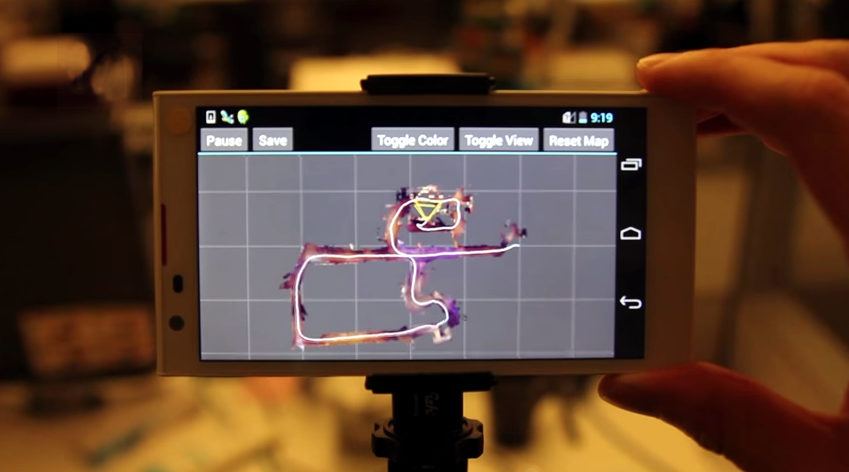
\includegraphics[width=1\textwidth]{img/mapdevice}
		 \caption{}
		 \label{fig:map_device}
	 \end{subfigure}
      	 \begin{subfigure}{0.39\linewidth} \centering
		 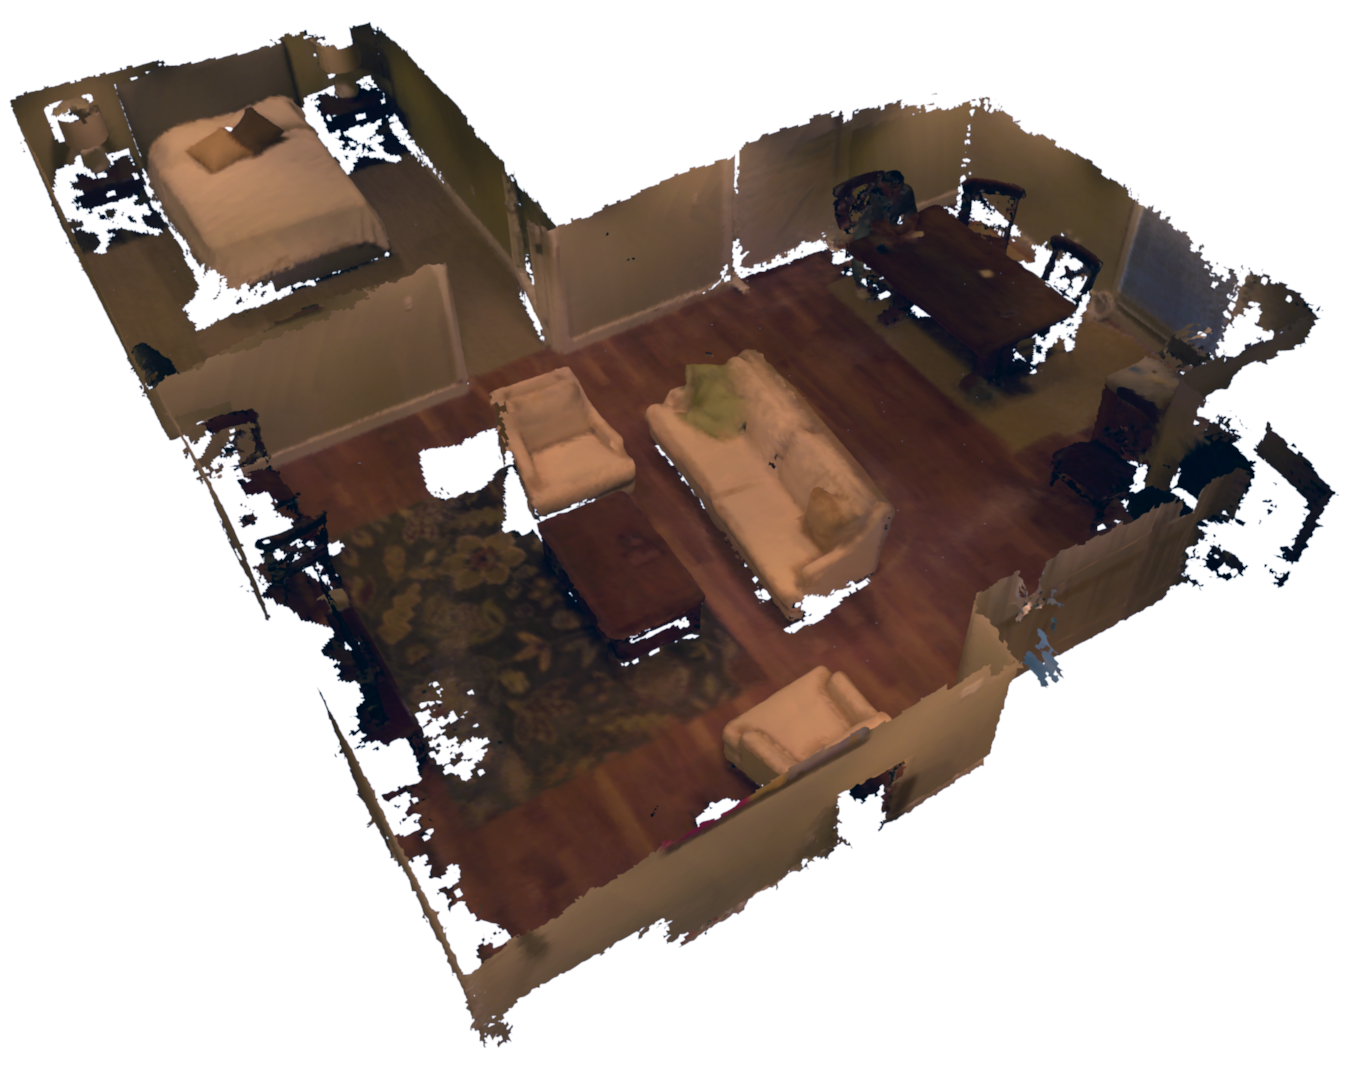
\includegraphics[width=1\textwidth]{img/apartment_scene_color.png}
		 \caption{}
		 \label{fig:apartment_color}
	 \end{subfigure}
      \caption{\figref{fig:map_device} shows our algorithm recording a map
      of an office building floor on a mobile device in real time, at a resolution of 3cm. A video of our approach running
  in real time is attached. \figref{fig:apartment_color} shows a
  reconstructed apartment scene at a resolution of 3cm exported from the
  device.}
  \label{fig:first_figure}
\end{figure*}


\begin{abstract}
Google's \textit{Project Tango}\cite{Tango} has made integrated depth sensing
and onboard visual-inertial odometry \cite{VINS} available to mobile devices such
as phones and tablets. In this work, we explore the problem of dense,
large-scale 3D realtime reconstruction on a mobile device with integrated
depth sensing. Solving this problem is a necessary pre-requisite for many indoor navigation, augmented
reality and indoor building scanning applications. State of the art approaches
in large-scale dense reconstruction \cite{Newcombe, Whelan2013} require large
amounts of memory and high-performance GPU computing, which is often
unavailable on mobile devices. Existing 3D reconstruction approaches on mobile
devices either only build a sparse reconstruction \cite{KleinSparse}, offload
their computation to other devices \cite{DTAM}, or require seconds-long
post-processing per frame \cite{TanskanenMetric}. Our approach trades off
resolution, color consistency, and pose drift for speed and memory
efficiency. By using chunked, dynamic spatial hash maps \cite{SpatialHashing}
of truncated signed distance volumes \cite{Curless1996}, we are able to
reconstruct and render very large (300 square meter) scenes at a resolution of
2-3cm in real time on a mobile device using only the CPU, with a memory
footprint that is approximately 84 percent smaller than \textit{Kinect Fusion}
\cite{Newcombe}. We provide both qualitative and  quantitative results on
publicly available RGB-D datasets \cite{FREIBURG}, and on datasets collected in
real-time from two devices.
\end{abstract}

\section{Introduction}
The task of real-time 3D reconstruction \cite{Hartley2004} is to extract the
true 3D geometry and color of a real scene from a sequence of noisy sensor readings
online. Solutions to this problem are useful for navigation, mapping, object
scanning, and more. The problem can be broken down into two components:
localization (\ie finding out where the sensor is), and mapping (\ie
reconstructing the scene geometry). Generally, localization is accomplished by a
combination of odometry \cite{VINS} and landmark-based localization
\cite{FastSlam}, and is efficiently solved by considering only a \textit{sparse}
representation of the world -- that is, as a collection of poses and landmark
associations. To be useful for high quality 3D reconstruction, mapping must in
contrast be \textit{dense}. That is, it must consider the full geometric
representation of the world either as surfaces, points, or volumes
\cite{Hartley2004}.  

Recently, mobile phone manufacturers have started adding
depth sensors to mobile devices, opening up the exciting potential for
real-time 3D reconstruction using a wireless, handheld device. In particular,
the devices we use in this work, Google's \textit{Project Tango} \cite{Tango}
phone and tablet use a small active infrared projection depth  sensor combined
with high-performance IMUs and a wide field of view camera (Sec.
\ref{section:hardware}) Other devices, such as the Occiptal Inc.
\textit{Structure Sensor} \cite{StructureSensor} have similar capabilities.  How
can we do real-time 3D reconstruction on these devices?

Consider house-scale (300 square meter) real-time 3D mapping and localization on
a \textit{Tango} device.  A user walks around a building, scanning the scene by
waving the device around. At house-scale, we are only concerned with features
at a resolution of about 2-3 cm (walls, floors, furniture, applicances, etc.).
To facilitate scanning, real-time feedback is given to the user on the device.
The user should be able to locate themselves inside the building, and should be
able to export the result after the scan is complete without losing any data.
\figref{fig:first_figure} shows an example of this use case in progress.

House-scale mapping on a mobile device requires that the 3D reconstruction
algorithm must run entirely on the device, and fast enough to allow user
interaction. Importantly, the entire dense 3D reconstruction must fit inside
the device's limited (2-4GB) memory. Because the mobile device might lack a
powerful discrete graphics processing unit (GPU), we will not be able to rely
on general purpose GPU computing to make the problem tractable in either
creating or rendering the 3D reconstruction.

Many state-of-the-art real-time 3D reconstruction algorithms \cite{Newcombe,
Whelan2013, WhelanLoopClose, Bylow2013} work by computing a truncated signed
distance field (TSDF) \cite{Curless1996} of the scene. The TSDF stores a
voxelized estimate of the distance to the nearest surface in the scene, up to a
fixed distance. While allowing for very high quality reconstructions, the TSDF
is very memory intensive. The size of the TSDF needed to reconstruct an entire
house may be on the order of several gigabytes  (Sec. \ref{section:memory}), and
rendering the resulting reconstruction in real-time would overwhelm the graphics
capabilities of the mobile device \textbf{(TODO: Justify this)}. Previous works
\cite{Whelan2013, WhelanLoopClose} have extended the TSDF to larger scenes by
storing a \textit{moving} voxelization and throwing away data incrementally --
but we are interested in preserving the volumetric data for later use.

We note in this work that most ( $\sim 85\%$) of the space occupied by
the TSDF in a typical scene is in fact empty (\figref{fig:memory_data}). Iterating over
empty space for the puposes of reconstruction and rendering wastes computation
time; and storing it wastes memory. Noting this fact, we introduce a novel
data structure, the Dynamic Spatially Hashed \cite{SpatialHashing} TSDF (Sec.
\ref{section:spatialhash}), which stores the distance field data as a two-level
structure in which static 3D \textit{chunks} of voxels are dynamically
allocated according to the presence of surfaces in the scene.
Because the data structure has $\mathcal{O}(1)$ access performance, we are able
to quickly identify which parts of the scene should be rendered, updated, or
deleted. This allows us to minimize the amount of time we spend on each depth
scan and keep the reconstruction running in real-time on the device. 

For localization, we use a mix of  visual-intertial odometry \cite{VINS} and
sparse keypoint-based mapping \cite{FastSlam} as a black box (Sec.
\ref{section:pose}). These approaches use only the 2D wide-angle camera and the
IMU, and take in no information from the depth sensor. As a consequence, our
approach is \textit{open-loop} in the sense that it does not attempt to explicitly estimate the pose of the sensor
from the 3D reconstruction. In spite of this limitation, we found that
using only open-loop visual odometry was sufficient to create high quality,
house-scale reconstructions (\figref{fig:overhead_night}).

 We provide qualitative and  quantitative results on publicly available RGB-D
 datasets \cite{FREIBURG}, and on datasets collected in real-time from two
 devices (Sec. \ref{section:experiments}). We compare different approaches for
 creating (Sec. \ref{section:scan_compare}) and storing (Sec.
 \ref{section:memory}) theTSDF in terms of memory efficiency, speed, and
 reconstruction quality.

\section{Related Work}
% \begin{itemize}
%     \item Real-time mapping solutions started with occupancy grids
%     \cite{Elfes1989}. But implemented in a naive way, these are too memory
%     intensive for our purposes. They are also bad at surface reconstruction.
%     \item More recent work in occupancy grid mapping reduces their memory
%     footprint by introducing an octree structure \cite{Wurm2010}. However,
%     octree structures have a hefty lookup time for each access, read, or write.
%     They also have poor cache performance during iteration.
%     \item \cite{Curless1996} introduced the TSDF as an efficient, accurate way
%     of reconstructing surfaces from many registered depth images. These are more
%     desirable for surface reconstruction than occupancy grids, because they
%     maintain local structure (inside vs. outside).
%     \item \cite{Newcombe}, introduced a method (Kinect Fusion) of creating and
%     registering TSDF volumes to depth images in real-time using ICP-like alignment of scans.
%     Making heavy use of GPU computing, Kinect fusion is able to generate and
%     display extremely high-quality reconstructions in a small area (due to
%     using a fixed size volume for reconstruction). 
%     \item Attempting to increase the size of Kinect Fusion reconstructions and
%     reduce drift, Kintinuous \cite{Whelan2013} keeps a running window of the
%     scene that gets integrated into a TSDF. Parts of the scene outside the
%     window are turned into a mesh with simple greedy triangulation. While this
%     allows them to make larger reconstructions than Kinect Fusion, they lose
%     distance field data as they move around the scene -- data which might still
%     be useful in its uncompressed form. We want to do large-scale reconstruction
%     \emph{without} compressing volumetric data into a surface representation
%     first.
%     \item Like \cite{Whelan2013}, \cite{Bylow2013} use the volume structure
%     directly to store colors. We copy the method of \cite{Bylow2013} to colorize
%     our meshes due to the simplicity and speed of the method.
% \end{itemize}
Mapping paradigms generally fall into one of two categories:
landmark-based (or \emph{sparse}) mapping, and high-resolution \emph{dense}
mapping \cite{FastSlam} . The distinction between the two is that sparse mapping
generates a metrically consistent map of landmarks based on key features in the
environment, while dense mapping globally registeredters all sensor data into a
high-resolution data structure. In this work, we are concerned primarily with
dense mapping, which is essential for high quality 3D reconstruction.

Because mobile phones typically have access only to 2D cameras, previous works
on dense reconstruction for mobile phones have gone to great lengths to extract
depth from a series of registered monocular camera images.  Early works on
real-time reconstruction and navigation on mobile devices relies on a spase
mapping, \cite{KleinSparse}, and is unable to produce dense 3D surface
reconstructions.  A recent algorithm by Tanskanen \etal
\cite{TanskanenMetric} generates impressive 3D reconstructions of small scenes
by means of monocular stereo computation and keypoint tracking. However,
because they \cite{TanskanenMetric} must intensively compute a depth map at
each frame by stereo, each frame capture still takes a few seconds, and only a
point cloud is stored. Another work by Newcombe \etal, Dense Tracking and
Mapping (DTAM) \cite{DTAM},  creates extremely high quality, dense 3D
reconstructions of scenes in real time using only a monocular camera -- while
the camera is attached to a high-performance desktop computer. Since our work
focuses on mobile devices with integrated depth sensors, such as the Google
\emph{Project Tango} devices \cite{Tango}, we luckily do not need to perform
costly monocular stereo as a pre-requisite to dense reconstruction. This allows
us to save our memory and CPU budget for the 3D reconstruction itself.

One of the simplest means of dense 3D mapping is to  store multiple registered
point clouds of the scene. While simple, point clouds fail to capture local
scene structure, are highly redundant, and noisy. Additionally, point clouds
fail to capture \emph{negative} information about the scene :  \ie, determining
which parts of the scene are empty. This information is crucial in situations
where the sensor is noisy, or has large patches of missing data \cite{Klingensmith2014}.

Elfes \cite{Elfes1989} introduced the concept of \emph{Occupancy Grid
Mapping}, which divides the world into a grid of voxels, each of which contains
an occupancy probability. Occupancy grids provide a principled alternative to
simple point clouds. They preserve local structure, and gracefully handle
redundant and missing data.  While more robust than point clouds, occupancy
grids suffer from aliasing, and lack information about surface normals and the
interior/exterior of obstacles.

% Attempts to extend occupancy grid maps to 3D have sometimes relied on octrees.
% Rather than storing a fixed-resolution grid, octrees store occupancy data in a
% spatially organized tree. In typical scenes, octrees reduce the required memory
% over occupancy grids by orders of magnitude. Octomap \cite{Wurm2010} is a
% popular example of the octree paradigm. However, octrees containing only
% occupancy probability suffer from many of the same problems as occupancy grids:
% they lack information about the interior and exterior of objects, and suffer
% from aliasing. Further, octrees suffer from logarithmic reading, writing, and
% iteration times, and have very poor memory locality characteristics.

Curless \cite{Curless1996} introduced an alternative to occupancy grids for 3D
reconstruction which, instead of storing the occupancy probability for each
voxel, stores an approximation of the signed distance field of the scene.  The
SDF is negative inside obstacles, and positive outside obstacles. The surface
is given implicitly as all points in space where the value of the SDF is zero.
The structure introduced in \cite{Curless1996} only maintains the distance
function within a small distance (called the \emph{truncation distance}) from
observed surfaces, and thus is called the Truncated Signed Distance Field
(TSDF).  While using more memory than occupancy grids, the TSDF creates much
higher quality surface reconstructions by preserving local structure.

The \emph{Kinect Fusion} \cite{Newcombe} algorithm uses a TSDF to
simultanesously extract the pose of a moving depth camera and the geometry of a
scene in real-time. Fusion solves the real-time 3D reconstruction problem
by using incremental estimates of the TSDF to inform the pose of the camera.
Making heavy use of the GPU for raycasting and rendering, Fusion is
capable of creating extremely high-quality, high-resolution surface 
reconstructions within a small area. However, like occupancy grid mapping, the
algorithm relies on a single fixed-size 3D grid of voxels, and thus is not
suitable for reconstructing very large scenes due to memory constraints.

The \emph{Kintinuous} \cite{Whelan2013} algorithm extends Kinect Fusion to
larger scenes by storing only a time-limited moving window of the TSDF in the
GPU. As the camera moves outside of the window, areas which are no longer
visible are turned into a surface representation. Hence, distance field data is
prematurely thrown away to save memory.

Our approach uses a TSDF as in\cite{Curless1996,Newcombe,Whelan2013,Bylow2013},
to store an estimate of the signed distance field of the scene. Unlike Kinect
Fusion, and like Kintinuous, we store a dynamic representation of the TSDF
which grows in size as the sensor travels through space. Unlike Kintinuous, we
do not prematurely throw away distance function data by converting it into a
mesh -- instead, we turn small areas of the scene into meshes for the purpose
of rendering, while \textit{preserving} the underlying distance field data. By
carefully considering what parts of the space should be turned into distance
fields at each timestep, we avoid needless computation and memory allocation in
areas far away from the sensor. 

\section{Approach} 
% \begin{itemize}
%     \item We start by getting an accurate probablistic model of the depth error
%     on the sensor by training a quadratic model of the depth and noise per
%     pixel. Depth images are compensated by this model before being passed into
%     our system.
%     \item We get pose by monocular visual-intertial odometry, rather than by
%     directly estimating pose from the depth image.
%     \item Depth comes in at 3-5Hz, as does RGB, but never at the same time.
%     \item Explain the TSDF
%     \item We represent the world as a collection of fixed size 16x16x16
%     \emph{Meta-Voxels} or \emph{Chunks}, aligned next to each other. Chunks are
%     allocated only when rays from the sensor would cause them to be updated.
%     They are garbage collected whenever there is no voxel with no weight in it.
%     \item To update a chunk with depth data, we can do one of two things:
%     \emph{Raycasting}, or \emph{Voxel Projection}. In the raycasting case, we
%     efficiently march rays through voxels in each updated TSDF volume, and
%     update the signed distance and weight there. In the voxel projection case,
%     we project the center of each voxel onto the image, and according to the
%     distance from the center of the voxel as compared with the depth from the
%     sensor, we either add weight to it, carve it, or do nothing to it.
%     \item Raycasting is O(number of rays), while Voxel Projection is O(number
%     of voxels). Voxel projection is an aliased approximation of raycasting. 
%     \item To do color, we project the points along the ray we are updating onto
%     the color image. We then update a separate \emph{Color Chunk} with data from
%     the RGB image.
%     \item We use a dynamic trunction distance based on the sensor model.
%     \item Rendering is handled by incrementally creating meshes of the updated
%     chunks using Marching Cubes. Chunks are frustum culled based on the frustum
%     of the renderer's camera, and only those which are near the camera and
%     inside its frustum are rendered. Faraway chunks are rendered as boxes. This
%     allows us to very efficiently render huge areas using only the fixed
%     function pipeline -- an important feature for devices with limited graphics
%     capability.
% \end{itemize}
\subsection{The Truncated Signed Distance Function}
\label{section:TSDF}
We will assume that the scene is static. Following Curless \cite{Curless1996},
we model the world as a volumetric function $\Phi(\mathbf{x}) : \mathbf{R}^3
\to \mathbf{R}$, where, for every 3D point in the world, we have its distance
to the nearest surface of an object. Inside objects, the value of $\Phi$ is
negative. Outside objects, the value of $\Phi$ is positive, and on the surface,
it is zero.

Consider the geometry of the ideal pinhole depth sensor. Rays emanate from the
sensor origin to the scene. At each timstep $t$ we have a set of rays
$Z_t$. Call the origin of the ray $o$, and the endpoint of the ray $\mathbf{x}$.
The length of the ray is given by $z = \|\mathbf{o}
- \mathbf{x}\|$. The direction of the ray is given by $\mathbf{\hat{r}} =
\frac{\mathbf{o} - \mathbf{x}}{z}$. The endpoint of each ray represents a point
on the surface. So if  the sensor is perfect, we know that the signed distance
function $\Phi(\mathbf{x}) = 0$ at that point. In practice, the ray is
corrupted by noise. Call $d$ the true distance from the origin of the sensor to
the surface along the ray. Then $z$ is actually a random variable drawn from a
distribution dependant on $d$ called the \textit{hit probability}
(\figref{fig:integration_diagram}).

The ray also implies that all the points in space along the ray from the sensor
origin up to the endpoint must be outside of any surface (or else the ray would
have been occluded by a a surface). Because real objects have non-zero
thickness, some part of the space along the ray beyond the endpoint will be
inside an object.

Further, very near the surface of the object, the signed distance function can
be approximated by the distance along the ray to the endpoint of  the ray
(\figref{fig:raycast_diagram}). Near $\mathbf{x}$, the signed distance function
is approximately the distance to $\mathbf{x}$. So, whenever $|u|$ is very
small:

\begin{equation} 
\label{eq:pointwise_tsdf} 
	\Phi(\mathbf{x} - u\mathbf{\hat{r}}) \approx u 
\end{equation}

The approximation is better whenever the ray is approximately
perpendicular to the surface, and worst whenever the ray is parallel to the
surface. Because of this, some works \cite{Bylow2013} instead approximate
$\Phi$ by locally fitting a plane around $\mathbf{x}$ using the neighboring
points and using the distance to that plane as a local approximation, \ie:

\begin{equation} 
\label{eq:planar_tsdf} 
	\Phi(\mathbf{x} - u\mathbf{\hat{r}}) \approx -u~\mathbf{\hat{r}} \cdot
	\mathbf{\hat{n}_x}
\end{equation}

\noindent where $\mathbf{\hat{n}_x}$ is the local surface normal around
$\mathbf{x}$. In general, the planar approximation (Eqn. \ref{eq:planar_tsdf})
is much better than the pointwise approximation (Eqn. \ref{eq:pointwise_tsdf}),
especially when surfaces are nearly parallel to the sensor -- but computing surface normals is not
always computationally feasible. In our work, we have chosen to use
the simpler pointwise approximation.

\begin{figure*}
   \begin{subfigure}{1.0\columnwidth}
     \centering
         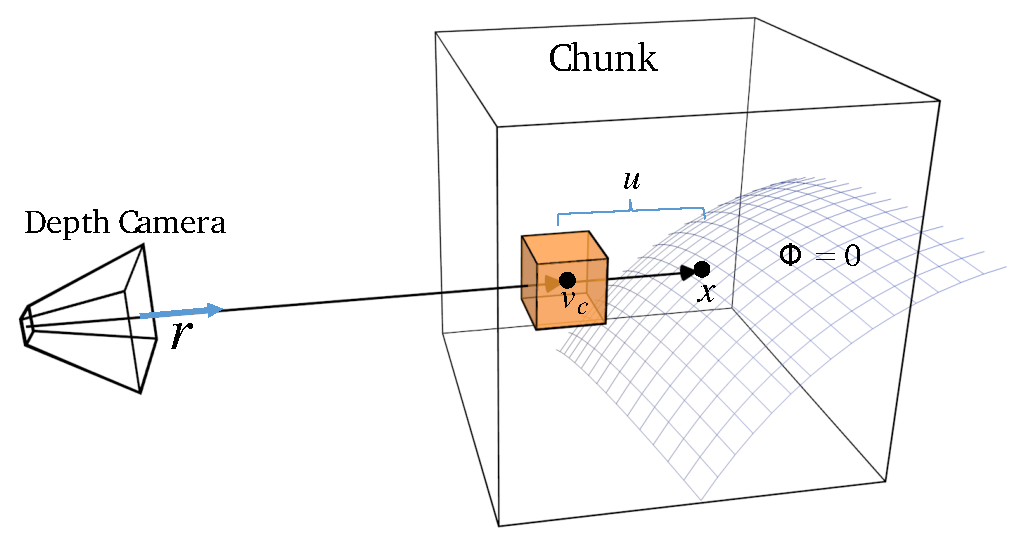
\includegraphics[width=1.0\textwidth]{img/Raycast}
      \caption{}
  \label{fig:raycast_diagram}
   \end{subfigure}
      \begin{subfigure}{1.0\columnwidth}
     \centering
         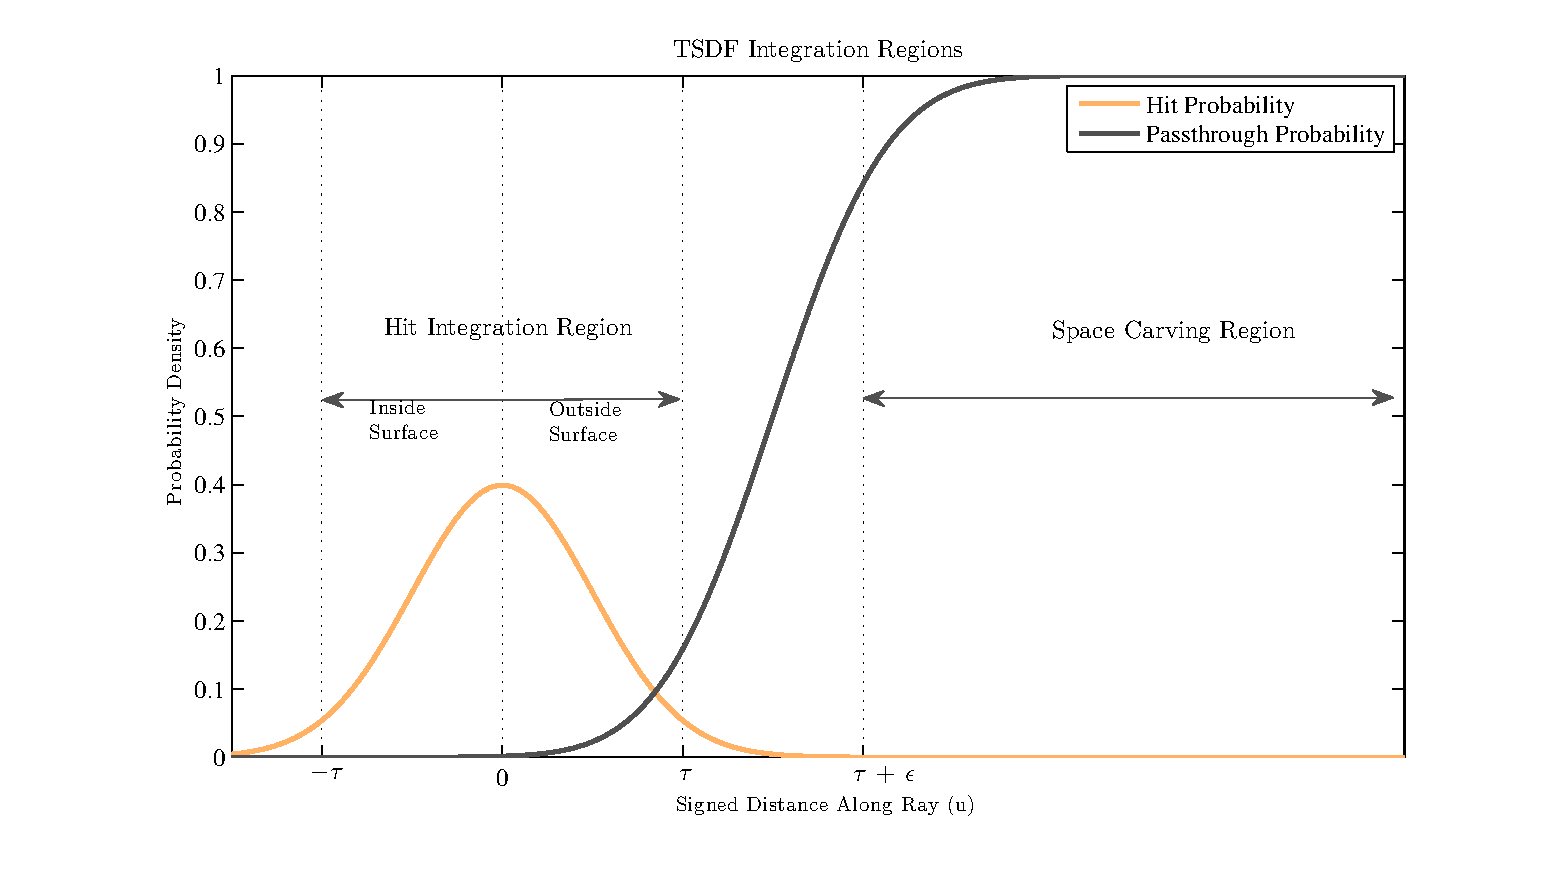
\includegraphics[ width=1.0\textwidth]{img/tsdf_integration.pdf}
         \caption{}
  \label{fig:integration_diagram}
   \end{subfigure}
   \caption{\figref{fig:raycast_diagram} is a diagram of a ray hitting a
   surface from the camera, and a voxel that the ray passes through. The length of the ray from the point at
      which the ray intersects the voxel and the surface, $u$, is an
      approximation of the signed distance function $\Phi$, when $u$ is small.
      \figref{fig:integration_diagram} shows a hypothetical plot of the
      hit probability of a ray $P\left(z - d = u \right) $, the pass
      probability $P\left(z - d < u\right)$, vs. $u$, where $z$ is the
      measurement from the sensor, and $d$ is the true distance from the sensor
      to the surface. The hit integration region is inside $[-\tau, \tau]$,
      wheras regions closer to the camera than  $\tau + \epsilon$ are in the space carving region (Section \ref{section:carving}). }
\end{figure*} 

This observation leads to the Truncated Signed Distance Function (TSDF)
\cite{Curless1996}. The TSDF is defined as:

\begin{equation}
	\Phi_{\tau}(\mathbf{x}) = 
	\begin{cases}
		\Phi(\mathbf{x}) &  \text{if} |\Phi(\mathbf{x})| < \tau \\
		\text{undefined} & \text{otherwise}
	\end{cases}
\end{equation}

\noindent where $\tau \in \mathbf{R}$ is the ``truncation distance'' in which
the TSDF is defined.

Following \cite{Curless1996}, to update the TSDF with a particular sensor
measurement, we update each voxel along the ray from $u = -\tau$ to $\tau$, and
take the weighted running average of distance field estimates over time. To do
this, we can introduce a global weighting function $W : \mathbf{R}^3 \to \mathbf{R}$ that represents the
confidence in the estimate of the TSDF at every point in space. A weight of $0$
corresponds to unknown space, wheras a weight of $\infty$ corresponds to space
where the distance to the nearest object is known with absolute certainty.

\begin{algorithm} 
	\caption{Truncated Signed Distance Function}
	\label{alg:TSDF}
	\begin{algorithmic}[1]
		\LineComment{For each timestep:} 
		\For {$t \in [1 \ldots T]$} 
			\LineComment{For each ray in the scan:} 
			\For {$\{\mathbf{o}_t, \mathbf{x}_t\} \in Z_t$} 
				\State {$z \gets   \|\mathbf{o}_t - \mathbf{x}_t\|$}
				\State {$\mathbf{r} \gets \frac{\mathbf{x}_t - \mathbf{o}_t}{z}$}
				\LineComment {Dynamic truncation distance.}
				\State{$\tau \gets \mathcal{T} (z)$} 
				\label{alg:line:dynamic_tsdf}
				\LineComment{Within the space carving region:}
			    \For{$u \in [\tau + \epsilon, z]$}
			    	\State {$\mathbf{v}_c \gets \mathbf{x} - u \mathbf{r}$}
			    	\If {$\Phi_{\tau}(\mathbf{v}_c) \leq 0$ }
				    	\State {$\Phi_{\tau}(\mathbf{v}_c) \gets \text{undefined}$}
				    	\label{alg:line:voxel_carve}
						\State {$W(\mathbf{v}_c) \gets 0$}
					\EndIf
			    \EndFor
				\LineComment{Within the hit region:}
				\For{$u \in [-\tau, \tau]$} 			 
					\State {$\mathbf{v}_c \gets \mathbf{x} - u \mathbf{r}$}
				   \LineComment{Update the TSDF and weight.}
					\State {$\Phi_{\tau}(\mathbf{v}_c) \gets \frac{ W(\mathbf{v}_c)
					\Phi_{\tau}(\mathbf{v}_c) + \alpha_{\tau}(u) u}{ W(\mathbf{v}_c)
					+\alpha_{\tau}(u)}$}
					\label{alg:line:tsdf_update}
					\State {$W(\mathbf{v}_c) \gets  W(\mathbf{v}_c)+ \alpha_{\tau}(u)$}
				\EndFor
			\EndFor
		\EndFor
	\end{algorithmic}
\end{algorithm}

The TSDF algorithm is outlined in Algorithm \ref{alg:TSDF}. It begins by
initializing the TSDF to an undefined value with a weight of $0$, then for each
depth scan, it updates the weight and TSDF value for all points along each ray
within the truncation distance $\tau$. The weight is updated according
to the scale-invariant weighting function $\alpha_{\tau}(u) : [-\tau,\tau]\to
\mathbf{R} $ for which the following holds:

\begin{equation}
	\forall \tau, \int_{-\tau}^{\tau} \alpha_{\tau}(u) du = K 
\end{equation}
 
 \noindent and $K$ is a constant. This is to ensure that changing the truncation
 distance does not change the speed at which the TSDF converges.  
 
Ideally, the weighting function should be determined by the hit probability of
the sensor and should correspond to the probability that $\Phi(\mathbf{x} - u
\mathbf{\hat{r}}) = 0$. It is possible \cite{Nguyen2012} to
directly compute the weight from the hit probability of the sensor; but in favor
of better performance, linear, exponential, and constant approximations of
$\alpha_{\tau}$ can be used \cite{Curless1996, Newcombe, Whelan2013, Bylow2013}.

Here, we simply use a constant approximation $\alpha_{\tau}(u) = \frac{1}{2
\tau}$, and use the hit probability of the sensor instead to  dynamically select
the value of $\tau$, as in \cite{Nguyen2012} (\figref{fig:integration_diagram}).
This results in poorer surface reconstruction quality in areas of high noise
than methods which more closely approximate the hit probability of the sensor.

\subsection{Colorization}
\label{section:color}
To create colored surface reconstructions, we use a method following Bylow
\etal \cite{Bylow2013}, also used in \textit{Kintinuous} \cite{Whelan2013},
which directly stores color information as volumetric data. Alongside the
truncated signed distance function, we store a volumetric color function
$C : \mathbf{R}^3 \to \mathbf{R}^3$, and a color weighting function
$W_{c} :
\mathbf{R}^3 \to \mathbf{R}$.

Color is updated in exactly the same manner as the TSDF. We assume that each
depth ray also corresponds to a color in the RGB space. We integrate along the
ray from $u \in [-\tau, \tau]$, and update the color:

\begin{align}
C(\mathbf{v}) \gets \frac{W_c(\mathbf{v}) C(\mathbf{v}) +
\alpha_c(u) \mathbf{c}}{W_c(\mathbf{v})}
\\
%
W_c(\mathbf{v}) \gets W_c(\mathbf{v}) + \alpha_c(u)
\end{align}

\noindent where $\mathbf{v} = \mathbf{x} - u\mathbf{\hat{r}}$ and $\mathbf{c}
\in \mathbf{R}^3$ is the color of the ray in color space, $\alpha_c$ is a color weighting function. In both \cite{Bylow2013} and
\cite{Whelan2013}, the color weighting function is proportional to the dot
product of the ray's direction and an estimate of the surface normal. But since
surface normal estimation is computationally expensive, we instead use the same
weight for both distance and color. The choice of color space (red/green/blue,
hue/saturation/value, etc.) depends on the application. As in \cite{Bylow2013}, we have chosen RGB space for the sake
of simplicity, at the expense of color consistency with changes in illumination.

% We must also deal with the fact that color images and depth data may be
% asynchronous. In our case, depth data is often delayed behind color data by as
% much as 30 milliseconds. So, for each depth scan, we project the endpoints of
% the rays onto the nearest color image in time to the depth image, disregarding
% occlusion, and use bilinear interpolation on the color image to determine the
% color of each ray.

\subsection{Dynamic Truncation Distance}
\label{section:dynamic_trunc}
Following the approach of Nguyen \etal\cite{Nguyen2012}, we use a dynamic
trunction distance based on the noise model of the sensor rather than a fixed
truncation distance. The truncation distance is given as a function of depth:

\begin{equation} \mathcal{T} (z) = \beta\sigma_{z} \end{equation}

\noindent where $\sigma_{z}$ is the standard deviation of the noise for a depth
reading of $z$, and $\beta$ is a scaling parameter which represents the number of
standard deviations of the noise we want to integrate over. Algorithm
\ref{alg:TSDF}, line \ref{alg:line:dynamic_tsdf} shows how this is used.

Using the dynamic truncation distance has the effect that further away from the
sensor, where depth measurements are less certain and sparser, depth
measurements are smoothed over a larger area of the distance field; while nearer
to the sensor, where depth measurments are more certain and closer together, the
truncation distance is smaller.

\subsection{Space Carving}
\label{section:carving}
When depth data is highly noisy and sparse, the relative importance of negative
data (that is, information about what parts of the space do not contain an
obstacle) increases over positive data \cite{Klingensmith2014}. Rays can be
viewed as \textit{constraints} on possible values of the distance field. Rays
passing through empty space constrain possible values of the signed distance
field to be positive at all points along the ray, wheras rays hitting objects 
only inform us about the presence of a surface very near the endpoint of the ray.

For this reason, we augment our TSDF algorithm with a \textit{space carving}
constraint. Along each ray within the space carving region (Fig.
\ref{fig:integration_diagram}), we clear away data that has a nonpositive stored
SDF. Algorithm \ref{alg:TSDF}, line \ref{alg:line:voxel_carve} shows how this is
accomplished. The effect is that as rays pass through previously integrated
regions of the TSDF, they clear away inconsistent data. Similarly, colors are
cleared away whenever rays pass through previously colored space.

Space carving gives us two advantages: first, it dramatically improves the
surface reconstruction in areas of very high noise (especially around the edges
of objects: see \figref{fig:dragon_closeup}), and second, it removes
some inconsistencies caused by moving objects and localization errors. If space
carving is not used, moving objects appear in the TSDF as permanent blurs, and
localization errors result in multiple overlapping isosurfaces appearing. With
space carving, inconsistent data is removed.

\subsection{Implementation: Spatially Hashed TSDF}
\label{section:spatialhash}
Each voxel contains an estimate of the signed distance function and an
associated weight. In our implementation, these are packed into a single 32-bit
integer. The first 16 bits are a fixed-point signed distance value, and the
last 16 bits  are an unsigned integer weighting value. Color is similarly
stored as a 32 bit integer, with 8 bits per color channel, and an 8 bit weight.
A similar method is used in \cite{Newcombe, Whelan2013, Bylow2013} to store the
TSDF.

Unfortunately, a flat volumetric representation of the world using voxels is
incredibly memory intensive. The amount of memory storage required grows as
$\mathcal{O}(N^3)$, where $N$ is the number of voxels per side of the 3D voxel
array. For example, at a resolution of $3\text{cm}$,  a $30\text{m}$ TSDF cube
with color would occupy 8 Gigabytes of memory. Worse, most of that memory would be
uselessly storing unseen free space.

For a large-scale real-time suface reconstruction application, a less
memory-intensive and more dynamic approach is needed. Confronted with this
problem, other approaches have either used  octrees \cite{Wurm2010}, or have
prematurely extracted isosurfaces from a moving TSDF volume to save memory
\cite{Whelan2013}. Neither of these approaches is desirable for our application.
Octrees, while maximally memory efficient, have significant drawbacks when it comes to
accessing and iterating over the volumetric data. An octree compresses
volumetric data by dividing the space recursively into octants. The leaves of
the tree contain the underlying volumetric data. Octants which contain no
leaves do not contain any allocated volumetric data. This allows the octree to
be incredibly memory efficient if the underlying volumetric data is sparse.

However, consider that every time an octree is \emph{queried},  a
logarithmic $\mathcal{O}(M)$ cost is incurred, where $M$ is the depth of the
Octree. In contrast, queries in a flat array are $\mathcal{O}(1)$.  If implemented na\"{\i}vely, an
octree will store pointers to child octants in each parent octant. The octants
themselves may be dynamically allocated on the heap. Each traversal through the
tree requires $\mathcal{O}(M)$ heap pointer dereferences in the worst case.
Even worse, adjacent voxels may not be adjacent in memory, resulting in very
poor caching performance \cite{CacheStructures}.

\begin{figure*}
  \centering
    \begin{minipage}{0.25\linewidth}
	 \begin{subfigure}{1.0\linewidth} \centering
			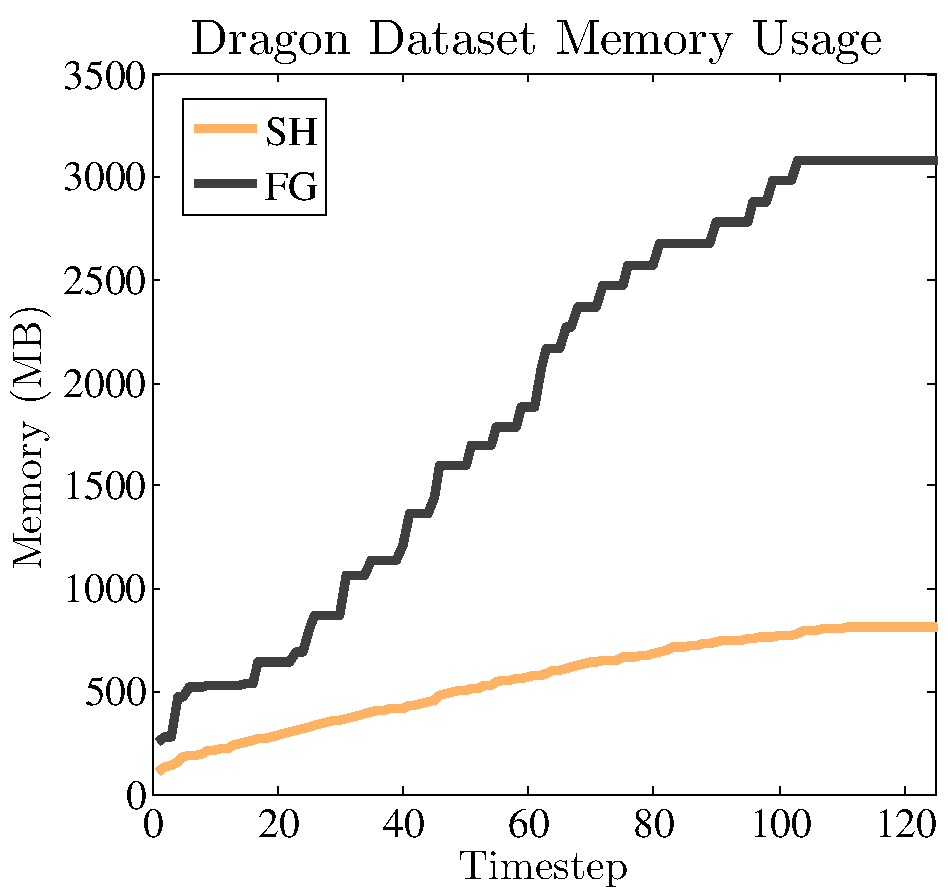
\includegraphics[width=1.0\textwidth]{img/memoryusage.pdf}
			 \caption{} 
			 \label{fig:memory_data}
		 \end{subfigure}  
		  \begin{subfigure}{1.0\linewidth} \centering
			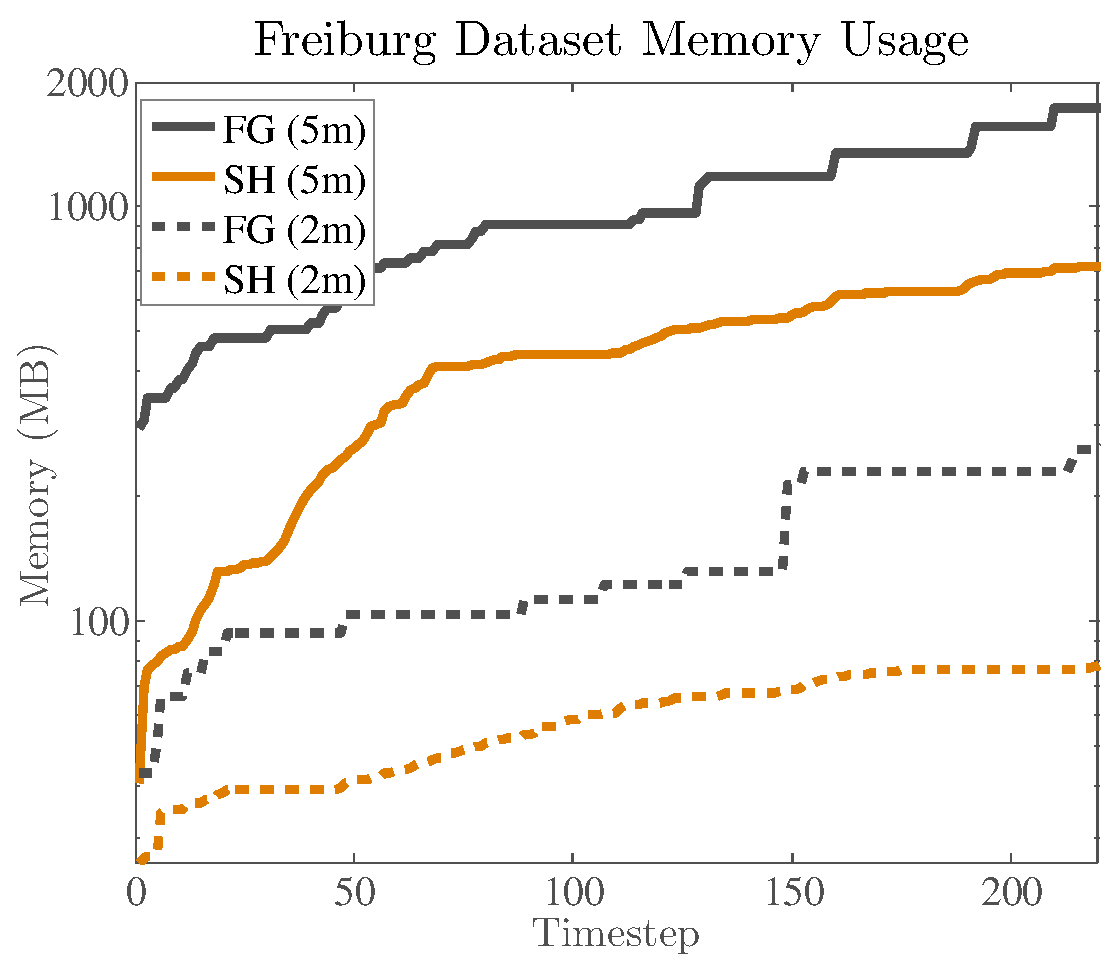
\includegraphics[width=1.0\textwidth]{img/memoryusage2.pdf}
			 \caption{} 
			 \label{fig:memory_data2}
		 \end{subfigure}
	 \end{minipage} 
	 \begin{minipage} {0.25\linewidth} 
	  \begin{subfigure}{1.0\linewidth} \centering 
		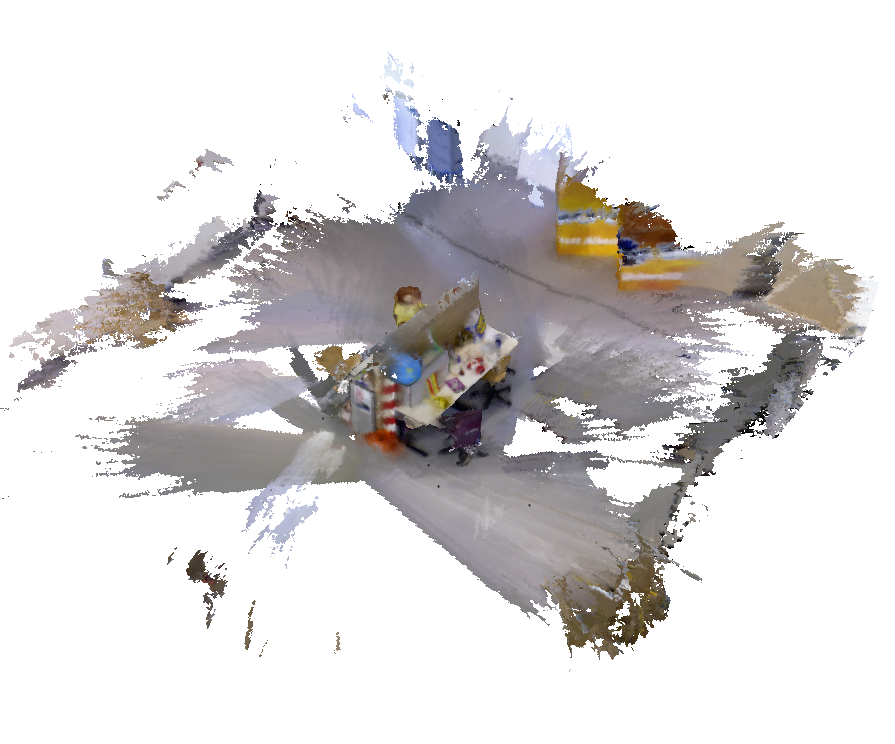
\includegraphics[width=1.0\textwidth]{img/freiburg_5m.png}
		 \caption{}
		 \label{fig:freiburg_5m}
	 	\end{subfigure} 
 		\begin{subfigure}{1.0\linewidth} \centering
		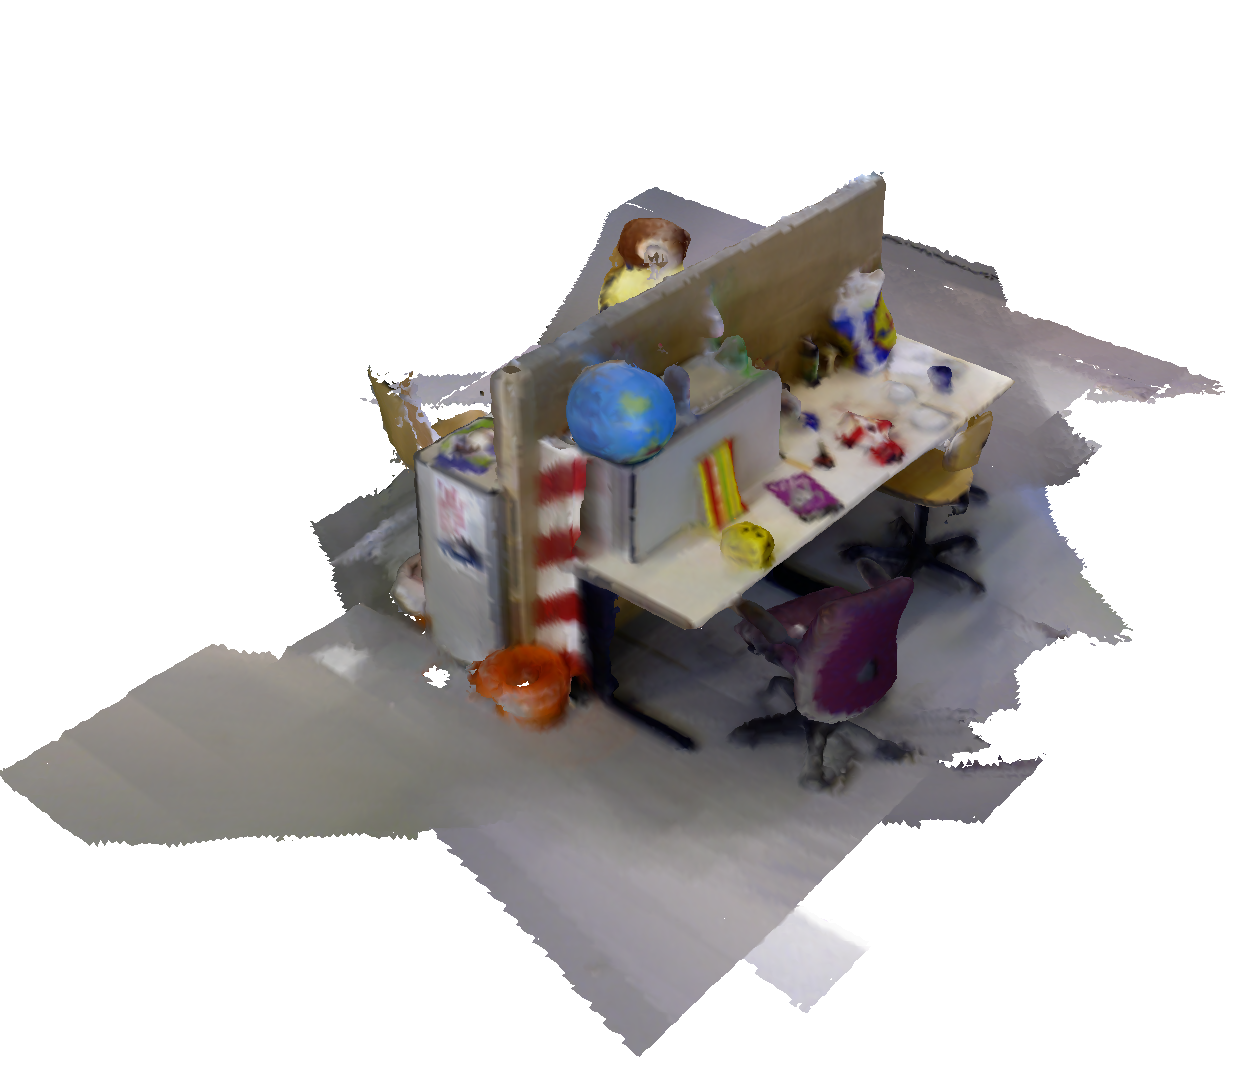
\includegraphics[width=1.0\textwidth]{img/freiburg_2m.png}
		 \caption{} 
		 \label{fig:freiburg_2m}
	 \end{subfigure}  
	 \end{minipage}
    \begin{minipage}{0.25\linewidth}
	  \begin{subfigure}{\linewidth} \centering
	      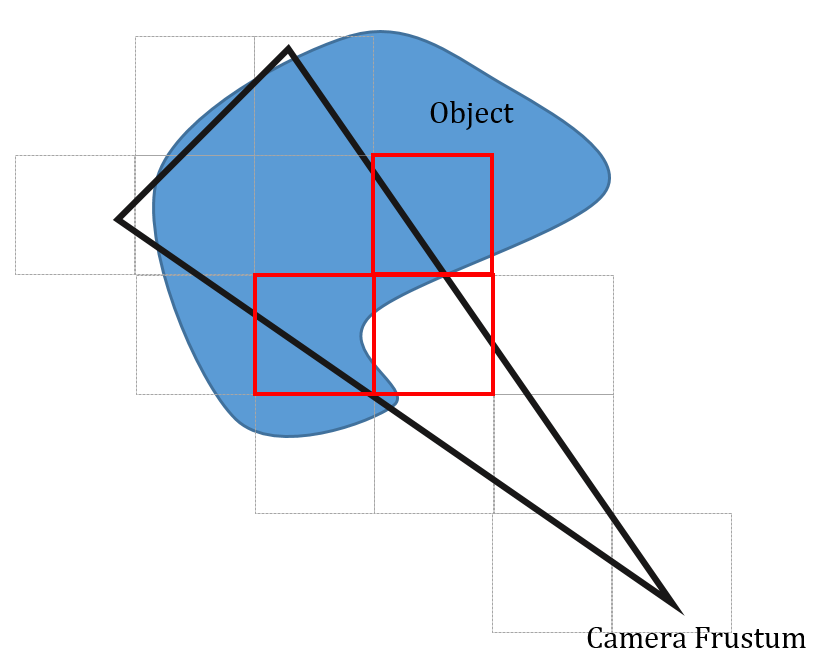
\includegraphics[width=1.0\textwidth]{img/frustum_cull}
	      \caption{}
	 	 \label{fig:frustum_cull}
	  \end{subfigure}
	  \begin{subfigure}{\linewidth} \centering
	    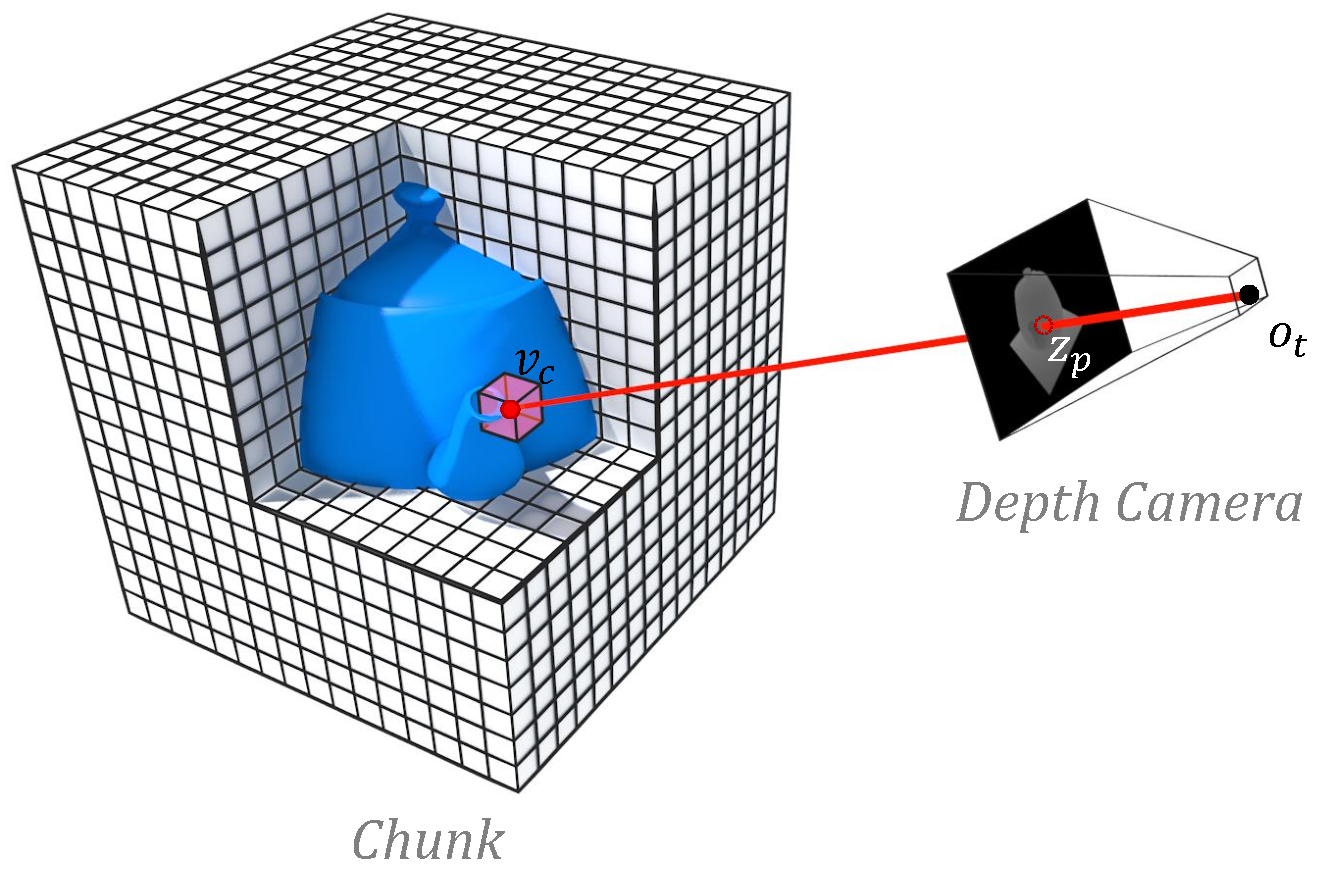
\includegraphics[width=1.0\textwidth]{img/projection_mapping}
	      \caption{} 
	      \label{fig:projection_mapping}
	  \end{subfigure} 
\end{minipage}
     \begin{minipage}{0.23\linewidth}
 	  	\begin{subfigure}{\linewidth} \centering
 	    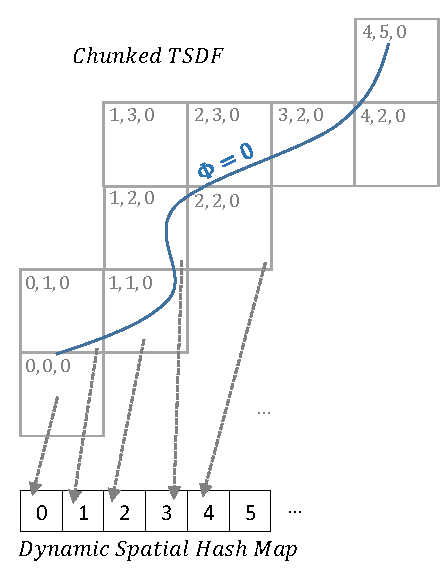
\includegraphics[width=1.0\textwidth]{img/chunks.pdf}
 	      \caption{}
 	  	\label{fig:chunks} 
 	  \end{subfigure} 
   \end{minipage}
  \caption{ We compare our spatial hashing (SH)
      approach to a na\"{\i}ve algorithm which simply allocates a monolithic
      block of volume memory for the entire space needed (FG) (Fig.
      \ref{fig:memory_data}).
      Memory is recorded for voxels of 3cm resolution, using both surface and
      color data. Chunks are of $16 \times 16 \times 16$ voxels. This figure
      does not account for the memory allocated for display meshes. We also collected memory
      usage statistics for the Freiburg \cite{FREIBURG} office dataset (Fig.
      \ref{fig:memory_data2}), varying the size of the depth frustum. Extending
      the depth frustum to 5 meters (\figref{fig:freiburg_5m}) results in a reconstructin of the entire
      room, wheras limiting the depth frustum to 2 meters (Fig.
      \ref{fig:freiburg_2m}) limits the reconstruction to the desk scene. Fig.
      \ref{fig:frustum_cull} shows all the TSDF chunks which intersect the depth camera frustum  and are within $\tau$ of a hit as green cubes. Only these
      chunks are updated when new data is received. The scene shown is a
      reconstruction of the Freiburg office \cite{FREIBURG} dataset at a
      resolution of 3cm. Fig \ref{fig:projection_mapping} shows a cutaway of a
      chunk containing an object. In projection mapping (Alg. \ref{alg:projection_mapping}),  a particular voxel with
      center $v_c$ is projected onto the depth camera at time $t$. The depth image is binlinearly interpolated to get
      $z_p$, a depth reading at the projected point. In \figref{fig:chunks}, chunks of voxels (grey) are allocated near
  the surface (blue) of the scene. Chunks are spatially hashed \cite{SpatialHashing} into a
      dynamic hash map. Lookups into the hash map are constant time. Within each
      chunk, voxels are allocated in a 3D array.}
\end{figure*} 

Instead of using an Octree, or a fixed 3D array (as in \cite{Newcombe,
Whelan2013}), we use a hybrid data structure which maintains some of the
advantages of both. We divide the world into a two-level tree. In the first
level we have \emph{chunks} of voxels (\figref{fig:chunks}). Each chunk consists of a
fixed grid of $N_c^3$ voxels, which are stored in a flat 3D array. Chunks are
allocated dynamically from a growing pool of heap memory as data is added, and
are indexed in a spatial 3D hash map \cite{SpatialHashing} by their spatial
coordinates. Following Teschner \emph{et. al} \cite{SpatialHashing}, we use the
hashing function:

\begin{equation}
\textbf{hash}(x, y, z) = p_1 x\oplus p_2 y \oplus p_3 z
~\text{mod}~n
\end{equation}

\noindent where $x, y, z$ are the 3D integer coordinates of the chunk, $p_1,
p_2, p_3$ are arbitrary, large primes, $\oplus$ is the xor operator, and $n$ is
the maximum size of the hash map.

Since chunks are a fixed size, querying data from the chunked TSDF involves
rounding (or bit-shifing, if $N_c$ is a power of two) a world coordinate to a
chunk and voxel coordinate, and then doing a hash-map lookup followed by a 3D
array lookup. Hence, querying is $\mathcal{O}(1)$. Further, since voxels within
chunks are stored adjacent to one another in memory, cache performance is
improved while iterating. By carefully selecting the size of chunks so that they
corresponding to $\tau$, we only allocate volumetric data near isosurfaces of
objects, and do not waste memory on empty space.

\subsection{Depth Scan Integration}
\label{section:scan_integration}
To perform the process described in Alg. \ref{alg:TSDF}, it is necessary
to consider each ray in each depth scan and upate each voxel
along the ray according to its distance to an observed surface. The most
straightfoward way of doing this is to simply iterate over each ray, and then
use a fast rasterization algorithm \cite{RayTracing} to determine which voxels
intersect with the ray. We will call this the Raycasting approach.
However, this approach is extremely computationally expensive, having a
performance bound by $\mathcal{O}(N_{\text{ray}} \times l_{\text{ray}})$, where
$N_{\text{ray}}$ is the number of rays in a scan, and $l_{\text{ray}}$  is 
proportional to the length of a ray being integrated. If we use a fixed-size
truncation distance and do not perform space carving, $l_{\text{ray}} = \tau$.
However, with space-carving, the length of a ray being integrated is
potentially unbounded.

A useful approximation of raycasting is \textit{projection mapping}. Used in
\cite{Nguyen2012, Bylow2013, Klingensmith2014}, projection mapping works by
projecting points in the voxel grid onto the depth image and comparing the depth value
there with the geometric distance from the center of the voxel to the camera
plane, and using that to approximate the distance along the ray from the camera
to the voxel. This is analogous to \textit{shadow mapping} \cite{Shadowmapping}
from computer graphics, where raycast shadows are approximated by projecting
onto a depth map from the perspective of the light source, except in our case, 
``shadows'' are regions occluded from the depth sensor.  Figure 
\ref{fig:projection_mapping} diagrams projection mapping, which is described in
Algorithm \ref{alg:projection_mapping}. Instead of iterating over each ray,
projection mapping iterates over each voxel. By projecting the voxel's center
onto the depth image, we can compare the actual depth reading to the distance
from the voxel's center to the camera origin as an approximation of the
distance to the surface, $u$. 

\begin{algorithm} 
	\caption{Projection Mapping}
	\label{alg:projection_mapping}
	\begin{algorithmic}[1]
		\LineComment{For each voxel in a chunk:} 
		\For {$\mathbf{v}_c \in V$}
		\State {$z \gets   \|\mathbf{o}_t - \mathbf{v}_c\|$}
		\LineComment{Project center onto depth image:}
		\State{$z_p \gets \mathbf{InterpolateDepth}(\mathbf{Project}(\mathbf{v}_c))$}
		\State{$u \gets z_p - z$} 
		\LineComment {Dynamic truncation distance.}
		\State{$\tau \gets \mathcal{T} (z_p)$} 
		\LineComment{Within the space carving region:}
	    \If{$u \in [\tau + \epsilon, z_p]$}
	    	\If {$\Phi_{\tau}(\mathbf{v}_c) \leq 0$ }
		    	\State {$\Phi_{\tau}(\mathbf{v}_c) \gets \text{undefined}$}
		    	\label{alg:line:voxel_carve}
				\State {$W(\mathbf{v}_c) \gets 0$}
			\EndIf
	    \EndIf
		\LineComment{Within the hit region:}
		\If{$u \in [-\tau, \tau]$} 			 
		   \LineComment{Update the TSDF and weight.}
			\State {$\Phi_{\tau}(\mathbf{v}_c) \gets \frac{ W(\mathbf{v}_c)
			\Phi_{\tau}(\mathbf{v}_c)+ \alpha(u) u}{W(\mathbf{v}_c) +\alpha(u)}$}
			\label{alg:line:tsdf_update}
			\State {$W(\mathbf{v}_c) \gets W(\mathbf{v}_c)+ \alpha(u)$}
		\EndIf
	\EndFor
	\end{algorithmic}
\end{algorithm}

Projection mapping has performance bounded by $\mathcal{O}(N_v)$, where $N_v$ is
the number of voxels affected by a depth scan. This value is nearly constant
over time, and depending on the resolution of the TSDF, may be significantly
less than the number of points. When using space carving (Section
\ref{section:carving}), raycasting has an additional performance hit bounded by
the length of the rays, wheras projection mapping does not suffer from this
performance hit. 

However, projection mapping suffers from resolution-dependant aliasing errors,
because the value of $u'$ taken from projection mapping may differ from the true
depth of the ray by up to the length of the diagonal of the voxel. Nuanced
surface information from many adjacent rays passing through a single voxel is
lost in the projection mapping case. This can be mitigated somewhat by
\textit{oversampling} each voxel (that is, considering many sampled points
inside each voxel) and taking the average projected depth over all the samples
-- but the speed of the approach decreases linearly with the number of 
additional samples taken. 

\subsection{Frustum Culling and Garbage Collection}
\label{section:frustum}
To determine which chunks should be updated by a depth scan, and which chunks
should be drawn, we use frustum culling. We first construct a conservative
geometric convex approximation of the space visible to the depth camera by
creating a camera frustum (\textit{i.e.} a truncated pyramid) with a far plane
at the maximum depth reading of the camera, and the near plane at the minimum
depth of the camera. We then take the axis-aligned bounding box of the camera
frustum in the global frame, and check each chunk inside the axis-aligned
bounding box for intersection with the camera frustum. Only those which
intersect the frustum are updated. 

Since the frustum is a conservative approximation of the space that could be
updated by a depth scan, some of the chunks that are visible to the frustum will
have no depth data associated with them. For this reason, we also store a flag
inside each chunk indicating whether or not that chunk ever contained the
endpoint of a ray from the depth camera (\figref{fig:frustum_cull}). Those
chunks which do not get updated during a depth scan are garbage collected
(deleted from the hash map), reducing memory overhead. Since the size of the
camera frustum is fixed, the garbage collection process has $\mathcal{O}(1)$
performance.

\subsection{Rendering}
\label{section:render}
In the original \textit{Kinect Fusion} work \cite{Newcombe}, rendering was
accomplished by raytracing on the GPU. Raytracing has the advantage of being a
pixel-perfect representation of the surface, and performance scales only with
the resolution of the rendering rather than with the size of the space. 
However, real-time raytracting requires intensive GPU computation that we
simply do not have on the mobile device. For that reason, it is necessary to
develop a real-time rendering solution that is amenable to the limited graphics
capabilities of mobile devices.

We take inspiration from some work in computer graphics for rendering large
natural terrains \cite{GPUGEMS3} using incremental Marching Cubes
\cite{Lorensen1987}. For each chunk, we store a triangle mesh.
Meshing is done asynchronously with the depth scan integration, and is
performed lazily. Triangle meshes are generated at the isosurface
$\Phi_{\tau}(\mathbf{x}) = 0$ whenever the chunk has been updated by a depth
scan since the last time the chunk was rendered. As in \cite{Bylow2013,
Whelan2013},  colors are computed for each vertex by trilinear interpolation of
the color map. At the borders of chunks, vertices are duplicated to reduce
co-dependence between the chunks, at the expense of causing slight seams
between chunk meshes. Only those meshes which are visible to the virtual camera
frustum are rendered. Meshes that are very far away from the camera are
rendered as a colored bounding box.

\subsection{Pose Estimation}
\label{section:pose}
We will assume we  have \textit{a priori} black-box pose estimation of
the sensor from a seperate tracking system. Specifically, in our experiments,
pose data is estimated from an onboard visual-intertial odometry system that
fuses data from a wide-angle camera, an intertial measurement unit, and a
gyroscope at 60 Hz using 2D feature tracking and an Extended Kalman Filter. A
more detailed discussion of this system can be found in \cite{VINS}. 

Unlike \textit{Kinect Fusion} \cite{Newcombe} and \textit{Kintinuous}
\cite{Whelan2013}, our approach makes no attempt to estimate the pose of the
sensor directly from depth data. Instead, we use depth data only for surface
reconstruction. Unfortunately, decoupling the pose estimation and surface
reconstruction results in failure to correct for drift in the pose estimation
using depth data, and can result in mis-alignment of depth scans.

% Section removed to save space
% \subsubsection{Pose Interpolation}
% We will assume that pose estimation, depth sensing, and color sensing are
% asynchronously executed, so we may not have all three measurements at a given
% time. To deal with asynchronous sensing and pose estimation, we linearly
% interpolate poses over time to determine the pose of a given sensor at any given time.
% 
% Call the global pose estimate of the sensor at time $t$,  ${H_{s}}^t$.
% Additionally, assume we have apriori extrinsic pose estimates for the color
% sensor ${E_{c}}$ and the depth sensor ${E_{d}}$. We are given a discrete
% trajectory of pose estimates from the visual-inertial odometry system:
% 
% $$ {H_{s}}^{t_1}, {H_{s}}^{t_2}, \ldots, {H_{s}}^{t_T} $$
% 
% Suppose at time $t'$, we get a color image. Assume that $t'$ is not represented
% in the list of sensor body poses. Then, either $t' < t_1$,  $t' > t_T$, or
% $t_a < t < t_b'$ for some $a, b \in [1, T]$. In the first case ($t' < t_1$), we
% disregard the color image. In the second case ($t' > t_T$), we wait until more data is
% acquired. In the third case, we would interpolate the pose of the color camera
% as:
% 
% $$ {H_{c}}^{t'} \approx E_c \cdot \textbf{Interp}\left(H_{s}^{t_a}, H_{s}^{t_b},
% \frac{t' - t_a}{t_b - t_a}\right) $$
% 
% Where $\textbf{Interp}$ is a function that  interpolates between two
% poses by linearly interpolating translation while spherically interpolating
% rotation, using $\frac{t' - t_a}{t_b - t_a} \in [0, 1]$ as an interpolation
% parameter. 

% Section removed to save space
% \subsection{User Interface}
% We developed a simple and intuitive prototype interface to test our approach on
% the device. Users were presented with options for controlling the resolution of
% the reconstruction, and were able to control when the system was active and
% inactive, allowing them to pause when moving objects obscured objects they were
% trying to model.
% 
% We present the user with camera controls as well. A virtual first person
% camera mimics the intrinsics of the depth camera. A third-person camera allows
% the user to rotate the virtual camera around their current position and get a
% better look at the quality of the reconstruction; and an orthographic overhead
% camera functions as a global map of where the user has been (Figure
% \ref{fig:map_device}).
% 
% At any time, the user can save the volumetric representation of the TSDF, or a
% surface mesh generated by marching cubes to disk.

 \begin{figure*} [htb]\centering
	 \begin{subfigure} {0.3\linewidth} \centering
		 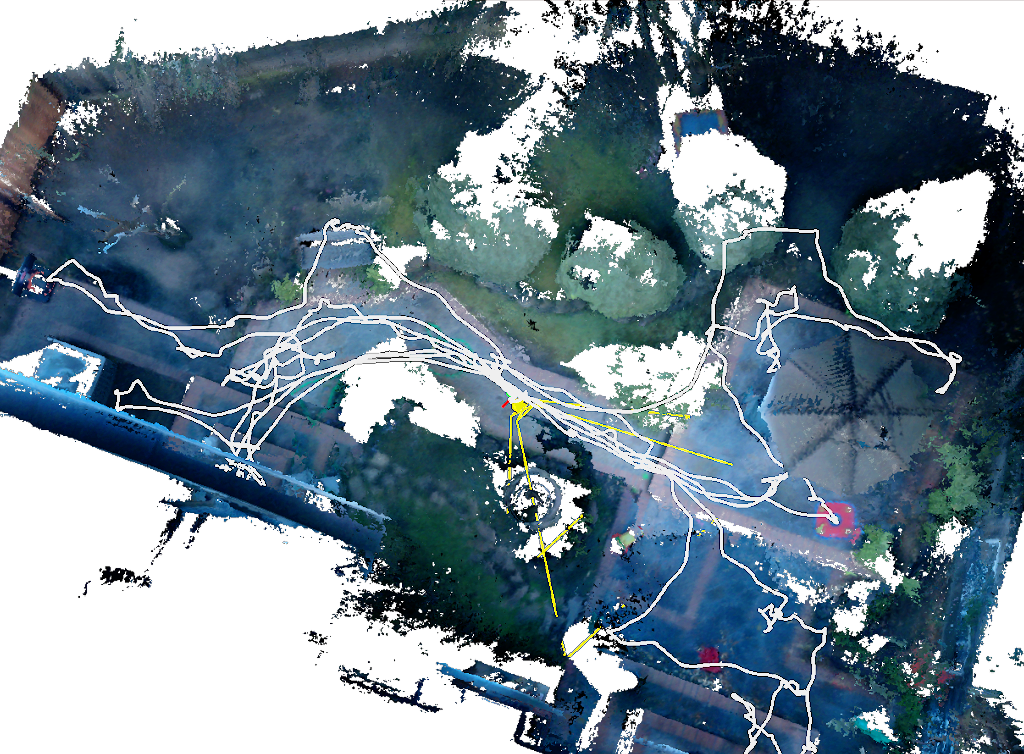
\includegraphics[width=1.0\textwidth]{img/colorbalance3}
		 \caption{}
		 \label{fig:overhead_night}
	 \end{subfigure}
	 \begin{subfigure}{0.3\linewidth} \centering
		 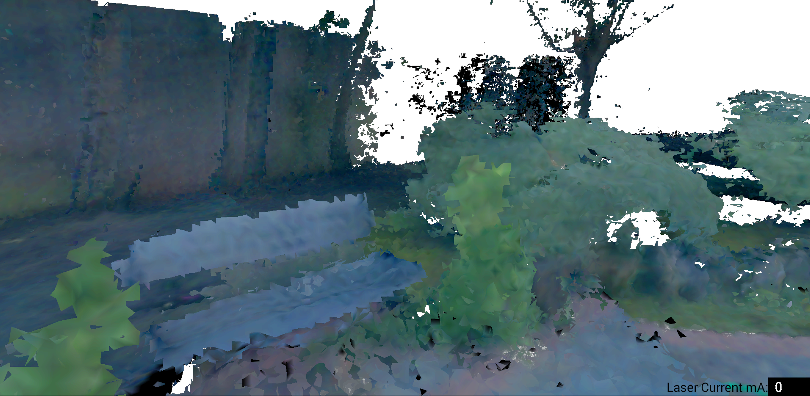
\includegraphics[width=1.0\textwidth]{img/colorbalance2}
		 \caption{}
		 \label{fig:night2}
	 \end{subfigure}
	 	 \begin{subfigure}{0.3\linewidth} \centering
		 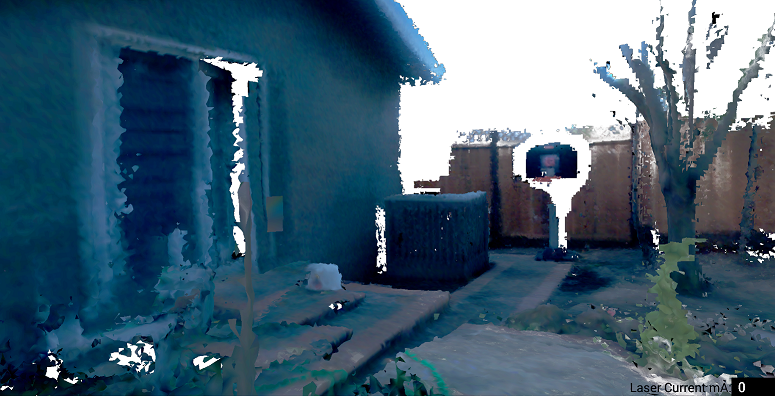
\includegraphics[width=1.0\textwidth]{img/colorbalance1} 
		 \caption{}
		 \label{fig:night3}
	 \end{subfigure} 
	 	 \begin{subfigure} {0.25\linewidth} \centering
		 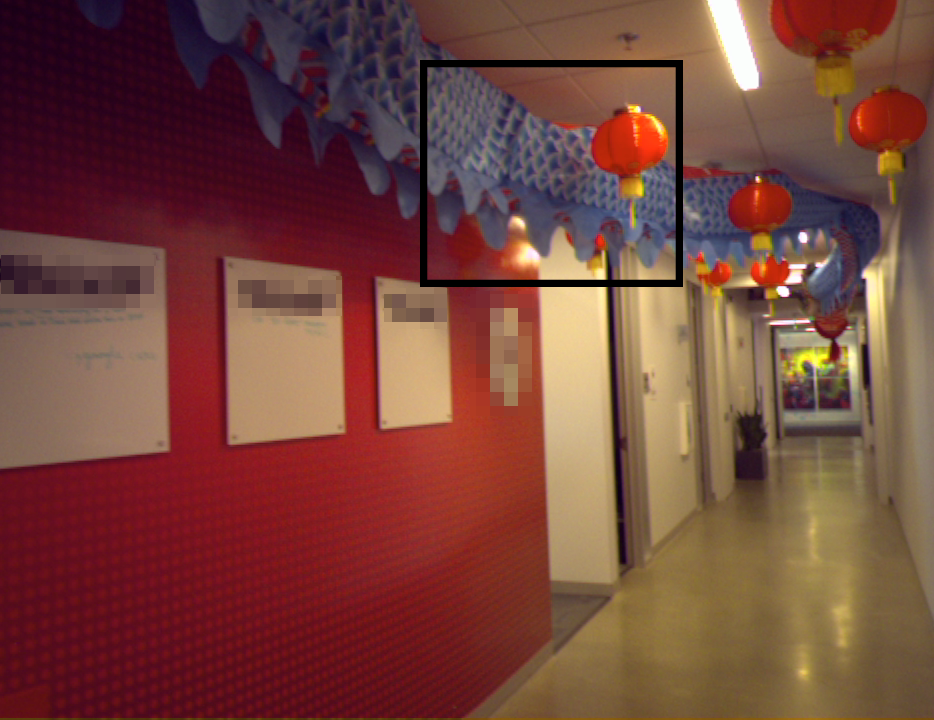
\includegraphics[width=1.0\textwidth]{img/dragon_color.png}  
		 \caption{}
		 \label{fig:dragon_color}
	 \end{subfigure}
	 	 \begin{subfigure}{0.3\linewidth} \centering  
		 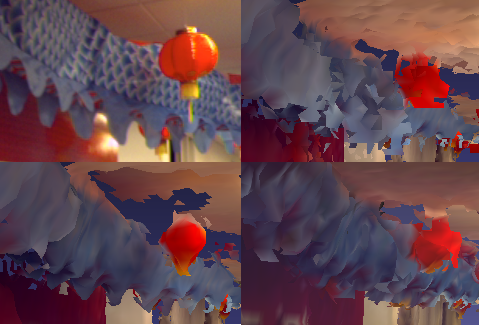
\includegraphics[width=1.0\textwidth]{img/dragon_closeup.png} 
		 \caption{}
		 \label{fig:dragon_closeup}
	 \end{subfigure} 
	  \begin{subfigure}{0.35\linewidth} \centering
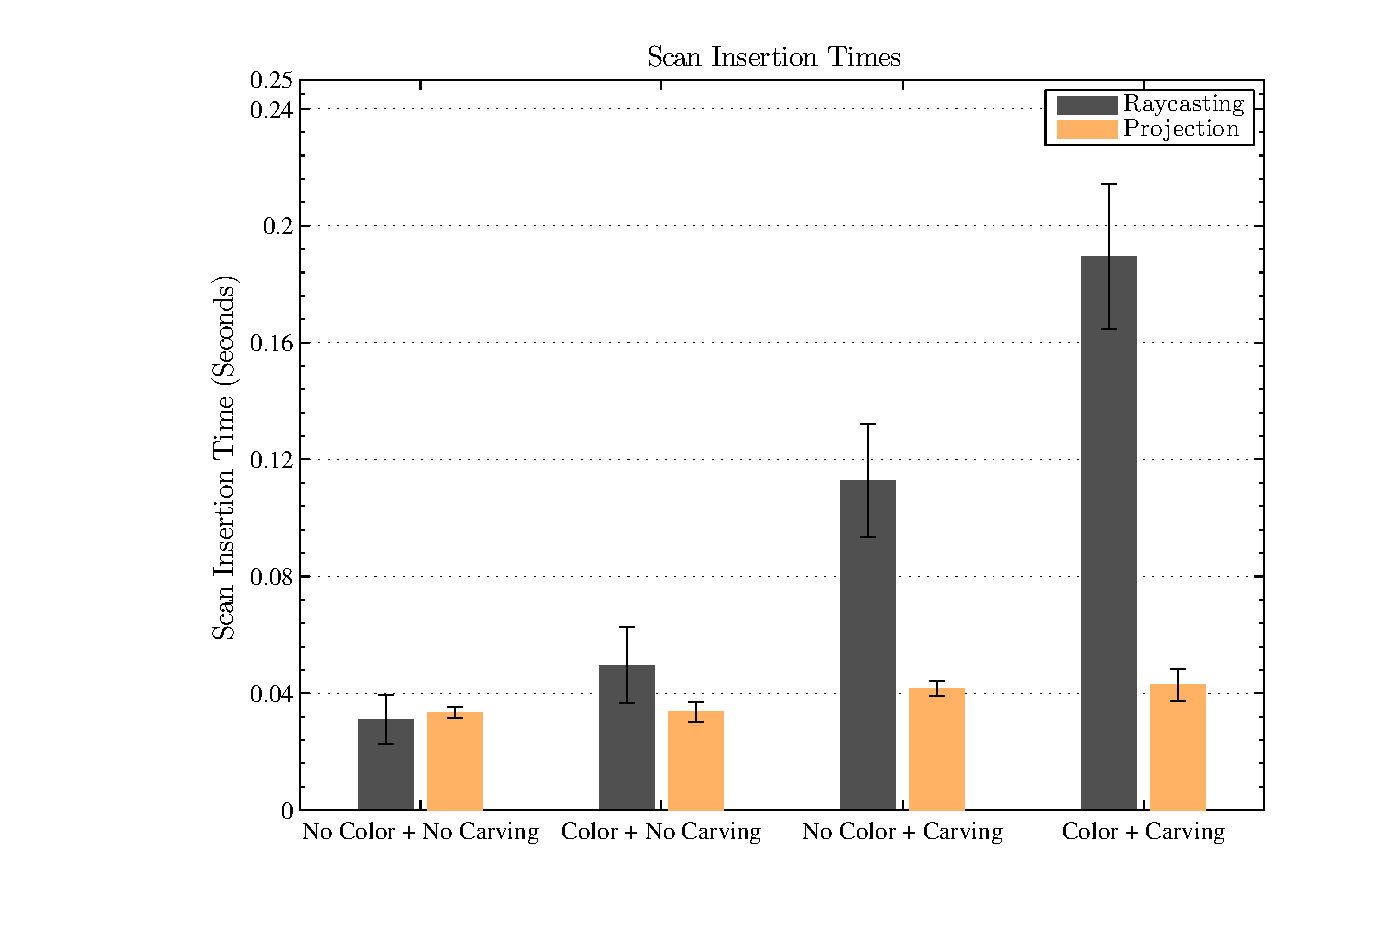
\includegraphics[width=1.0\textwidth]{img/timing_data.pdf}
		 \caption{}
		 \label{fig:timing}
	 \end{subfigure} 
	 \caption{\figref{fig:overhead_night} shows an overhead view of
	 an outdoor scene captured at night with the yellowstone device at a
	 resolution of 3 cm. The yellow pyramid represents the depth camera frustum. The white
	 lines are the aggregate trajectory of the device. Figures \ref{fig:night2}
	 and \ref{fig:night3} show closeups of the scene taken live from the device.
	 The scene was captured using projection mapping (Sec.
	 \ref{section:scan_integration}), without space
	 carving (Sec. \ref{section:carving}). Different depth scan integration techniques are compared. Fig.
	 \ref{fig:dragon_color} shows the color image for reference.  Fig.
	 \ref{fig:dragon_closeup} is a closeup of a lantern in the scene; 
	 counter-clockwise from the top left: color image, projection mapping without
	 space carving, projection mapping with space carving, and raycasting without
	 space carving. During the scan, the user was looking mostly toward the
	 ceiling, at the colorful dragon. \figref{fig:timing} shows
      scan insertion times for each of the methods as recorded on a desktop
      computer.}
	 \label{fig:device_data}
 \end{figure*} 


\section{Experiments and Results}
\label{section:experiments}
\subsection{Hardware}
\label{section:hardware}
We implemented our approach on two devices: a \textit{Project Tango}
``Yellowstone" tablet device, and a \textit{Project Tango} ``Peanut'' mobile 
phone device. The phone device has 2GB of RAM, a quadcore
CPU, a six-axis gyroscope and accelerometer, a wide-angle $120^\circ$ field of
view tracking camera which refreshes at 60Hz, a projective depth sensor which
refreshes at 6Hz, and a 4 megapixel color sensor which refreshes at 30Hz. The
tablet device has 4GB of ram, a quadcore CPU, an Nvidia Tegra K1 graphics card,
an identical tracking camera to the phone device, a projective depth sensor
which refreshes at 3Hz, and a 4 megapixel color sensor which refreshes at 30Hz.
%Devices were depth calibrated \ref{subsection:calibration} prior to testing. 

%  \subsection{Sensor Calibration}
% \label{subsection:calibration}
% The depth image may be corrupted by noise, feature nonlinear distortions, and
% have large segments of missing data. Our noise model of the sensor will consider
% Gaussian noise on the depth, and per-pixel quadratic distortion. Call a
% particular depth reading from the device the random variable $D$, and the true
% depth of the scene at that point $z$. Then we have the model:
%  
%  \begin{equation}
%  	D = z + a{z}^2 + b z + c+ \epsilon(z)
%  	\label{eqn:distort}
%  \end{equation} 
%  
%  \noindent where $a, b, c$ are coefficients of a quadratic depth distortion
%  model, and $\epsilon(z)$ is a random variable drawn from the parametric
%  Gaussian distribution function $\mathcal{N}(z, \sigma(z))$.
%  That is, the distribution is mean-centered on $z$, and has a depth-dependant
%  standard deviation $\sigma(z)$.
%  
%  We have found that on the \textit{Tango}  Peanut \cite{Tango} device, the
%  nonlinear distortion is very severe. At a distance of 3 meters, the reading
%  can be distorted by as much as 30 centimeters. Depth distortion on the
%  Yellowstone device is comparably negligible.  To get an accurate
%  reconstruction of the world, it is critical to correct for this distortion.
%  This is done by inverting the distortion model (Eqn. \ref{eqn:distort}) to
%  estimate the true depth $z$ from the distorted reading $D$.
%   
%  \begin{figure} \centering
% 	 \begin{subfigure} {0.3\columnwidth} \centering
% 		 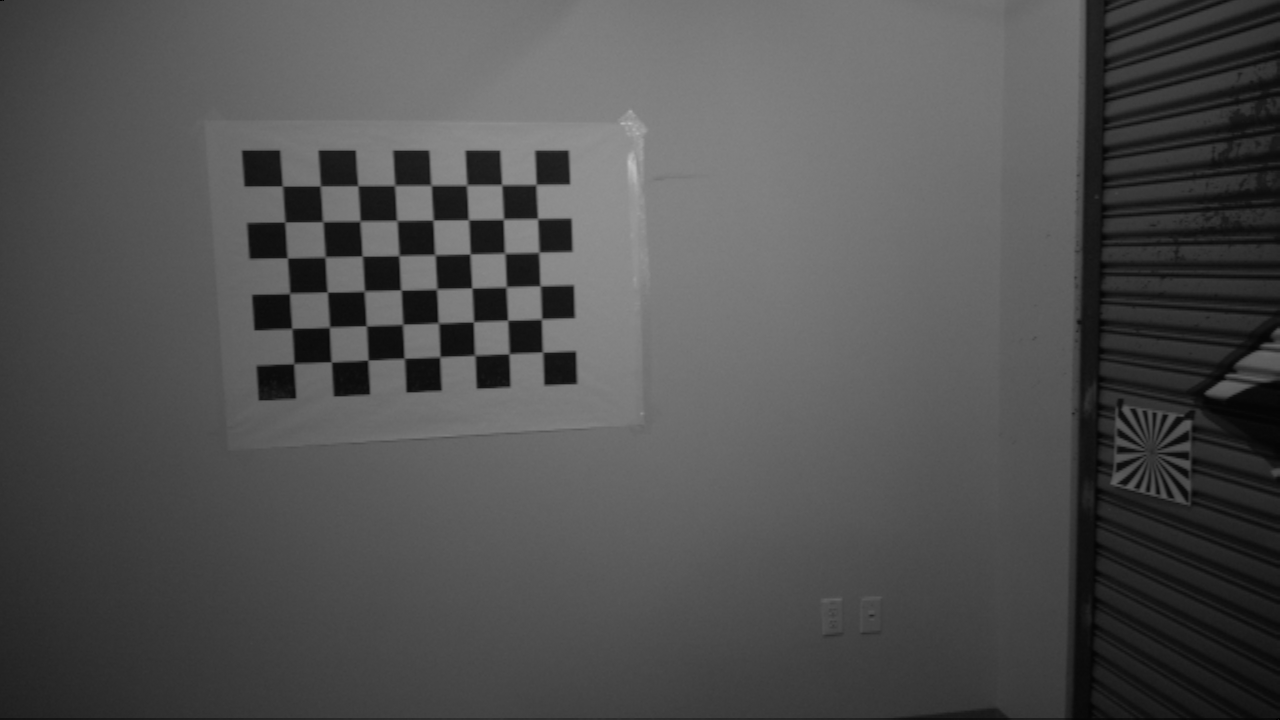
\includegraphics[width=1.0\textwidth]{img/calibration_grey}
% 		 \caption{}
% 	 \end{subfigure}
% 	 \begin{subfigure}{0.3\columnwidth} \centering
% 		 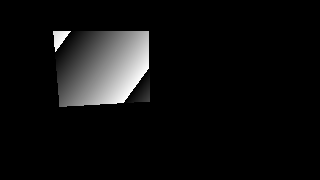
\includegraphics[width=1.0\textwidth]{img/calibration_model}
% 		 \caption{}
% 	 \end{subfigure}
% 	 	 \begin{subfigure}{0.3\columnwidth} \centering
% 		 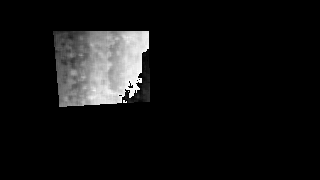
\includegraphics[width=1.0\textwidth]{img/calibration_data}
% 		 \caption{}
% 	 \end{subfigure}
% 	 \caption{Components collected in our calibration procedure. The greyscale (a)
% 	 image is used to compute a linear plane model (b) for depth. That model is
% 	 compared to the actual depth data (c) over a series of checkerboard poses.}
% 	 \label{fig:calibration}
%  \end{figure}
%  
%  To train the distortion and noise model, we first calibrate the sensor with the
%  use of a checkerboard calibration target. Images of the target are taken at
%  multiple distances and angles from the camera (\figref{fig:calibration}). We
%  fit an ideal plane to the target to determine what the true distance should be
%  at each pixel. Then, we perform quadratic regression on the depth readings
%  against the predicted readings from the plane to find the per-pixel distortion
%  coefficients. The function $\sigma(z)$ is computed in a similar way, by
%  computing a histogram of standard deviations of the depth readings, and then
%  performing quadratic regression on the result. A single function $\sigma(z)$ is used for the
%  entire image, unlike the distortion model which is computed on a per-pixel
%  basis.
%  
\subsection{House Scale Online Mapping}
\label{section:mapping}
Using our algorithm, we are able to create and display large scale maps at a
resolution as small as 2cm in real-time using only visual-intertial odometry for
pose estimation. \figref{fig:map_device} shows a map of an office building floor
being reconstructed in real-time using the phone device. This scenario is also
shown in an attached video. Using the tablet device, we have reconstructed
(nightime) outdoor scenes in real-time (\figref{fig:overhead_night}).

In the course of online mapping, the user has immediate feedback on model
completeness, and can pause mapping for live inspection. The system continues
localizing the device using visual-intertial odometry even when the mapping is
paused. After mapping is complete, the user can save the map to disk.
 
\subsection{Comparing Depth Scan Integration Algorithms} 
\label{section:scan_compare}
We implemented both the raycasting and voxel projection modes of depth scan
integration (Sec. \ref{section:scan_integration}), and compared them in terms of
speed and quality. We found that projection mapping was far more efficient than
raycasting when space carving was used (\figref{fig:timing}). However,
projection mapping results undesirable aliasing artifacts; especially on
surfaces nearly parallel with the camera's visual axis. Additionally, color consistency suffers
with projection carving, because rather than color being averaged by all the
rays passing through each voxel, only a single color is used for each projected
voxel center. The use of space carving drastically reduces noise artifacts,
especially around the silhouettes of objects (\figref{fig:dragon_closeup}). We
note that using both space carving \emph{and} raycasting is not fast enough for real-time mapping on the device
using our approach.

\subsection{Memory Usage}
\label{section:memory}
We additionally compared memory usage statistics of our chunked approach to a
na\"{\i}ve approach which allocates a single block of memory to tightly fit the
entire volume explored (\figref{fig:memory_data}). As the size of the space
explored increases, our approach uses about a tenth as much memory as the
na\"{\i}ve approach. This is because the majority of the space explored contains no
surfaces. Notice that in \figref{fig:memory_data}, the na\"{\i}ve approach uses
nearly 300MB of RAM wheras our approach never allocates more than 47MB of RAM
for the entire scene, which is a 15 meter long hallway.

We tested our approach on the publicly available Freiburg RGB-D dataset
\cite{FREIBURG}, which contains ground truth pose information from a motion
capture system (\figref{fig:freiburg_2m}). In the Freiburg office dataset, a
\textit{Kinect} sensor makes a loop around a central desk scene. The room is
roughly 12 by 12 meters in area.  Memory usage statistics (Fig.
\ref{fig:memory_data2}) reveal that when all of the depth data is used
(including very far away data from the surrounding walls), a na\"{\i}ve fixed grid
approach would use nearly 2GB of memory at a 2cm resolution, wheras our
approach uses only around 700MB. When the depth frustum is cut off at 2 meters
(mapping only the desk structure without the surrounding room), our approach
uses only 50MB of memory, wheras the na\"{\i}ve approach would use nearly 300MB.

% \subsection{Limitations due to Odometry Drift}
% Since we do not update pose using depth data, odometry pose drift severely 
% corrupts the map, especially when the same area is repeatedly scanned . We  
% compare the map produced online using visual-inertial odometry to one produced
% offline by first correcting the pose of the camera using bundle adjustment (a
% process which takes several hours) to show the effect of drift  (Figure
% \ref{fig:bundleadjust}). Double walls, accidentally carved space, and other
% artifacts result when drift is present. Clearly, this limitation presents the
% need for dense loop closure and alignment. High quality meshes produced using
% offline bundle adjustment for pose estimates are shown in figure
% (\ref{fig:apartment}).
% 
%   \begin{figure*} \centering
% 	 \begin{subfigure} {0.49\columnwidth} \centering
% 		 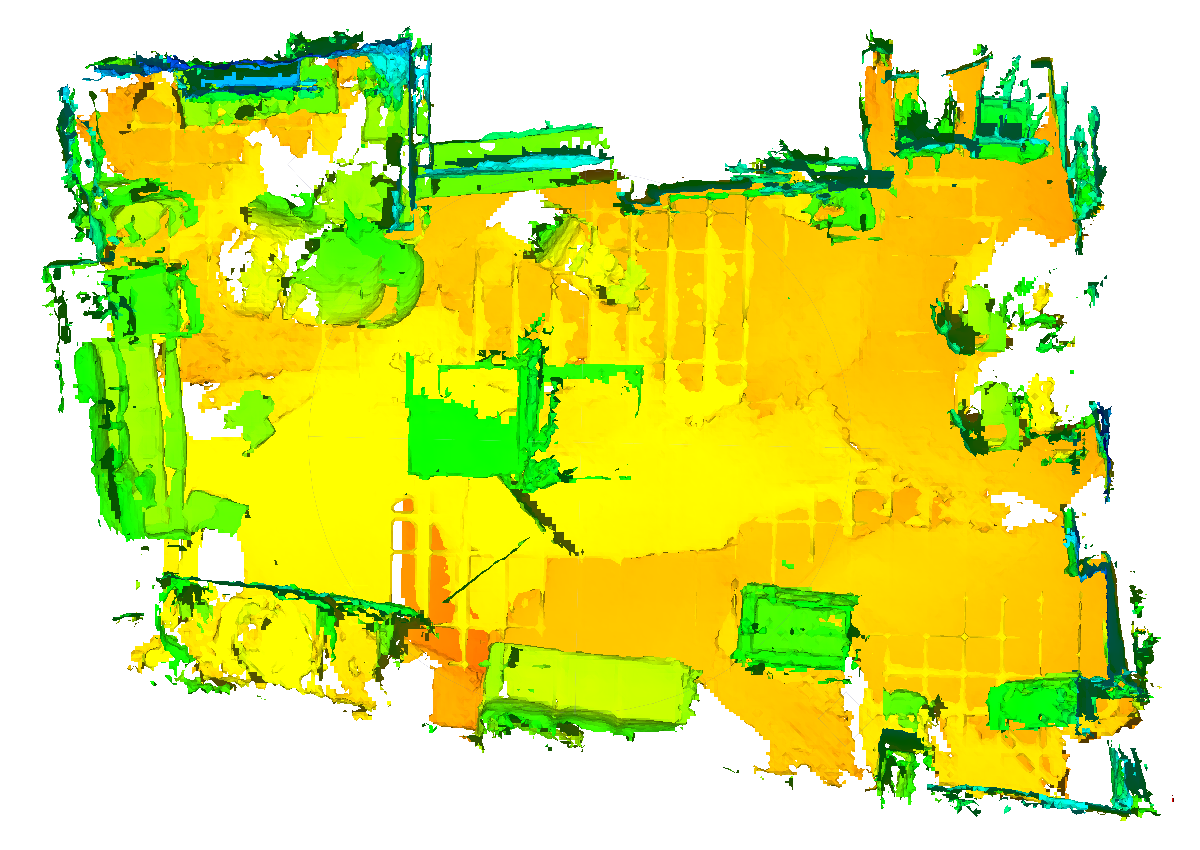
\includegraphics[width=1\textwidth]{img/gameroom_vio.png}  
% 		 \caption{}
% 		 \label{fig:gameroom_vio}
% 	 \end{subfigure}
% 	 \begin{subfigure}{0.49\columnwidth} \centering
% 		 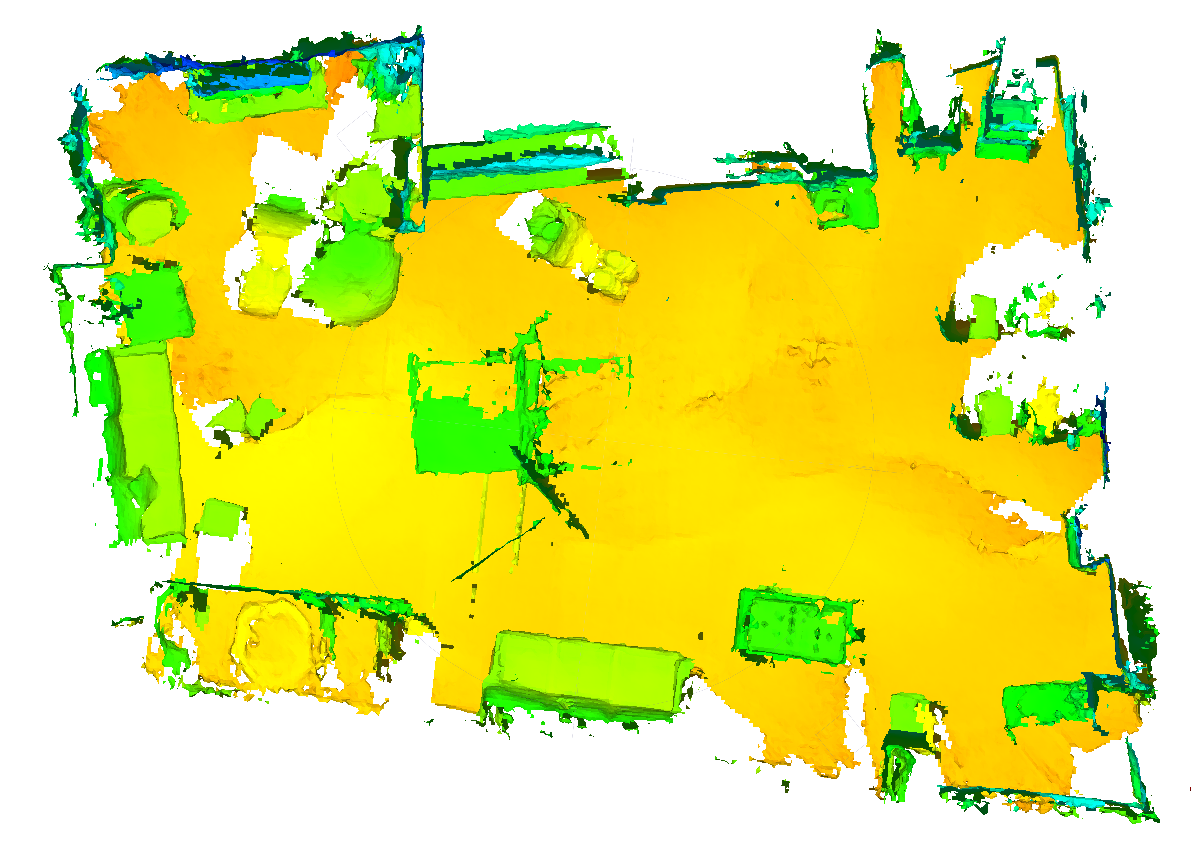
\includegraphics[width=1\textwidth]{img/gameroom_bundleadjust.png}
% 		 \caption{}
% 		 \label{fig:gameroom_bundleadjust}
% 	 \end{subfigure}
% 	 \caption{The phone device was used to scan a midsized room by walking in a
% 	 loop around the room three times. A top down view is shown. Meshes are colored
% 	 with respect to their height; the floor is orange and objects green. Drift
% 	 from visual-inertial odometry causes severe corruption and artifacts in the 
% 	 TSDF (\ref{fig:gameroom_vio}). By pre-processing the trajectory offline using
% 	 bundle adjustment, we can produce a much higher quality mesh using the same
% 	 dataset (\ref{fig:gameroom_bundleadjust}). Meshes are produced using
% 	 raycasting and space carving. }
% 	 \label{fig:bundleadjust}
%  \end{figure*}  
%  
%    \begin{figure*} \centering
% 	 \begin{subfigure} {0.49\columnwidth} \centering
% 		 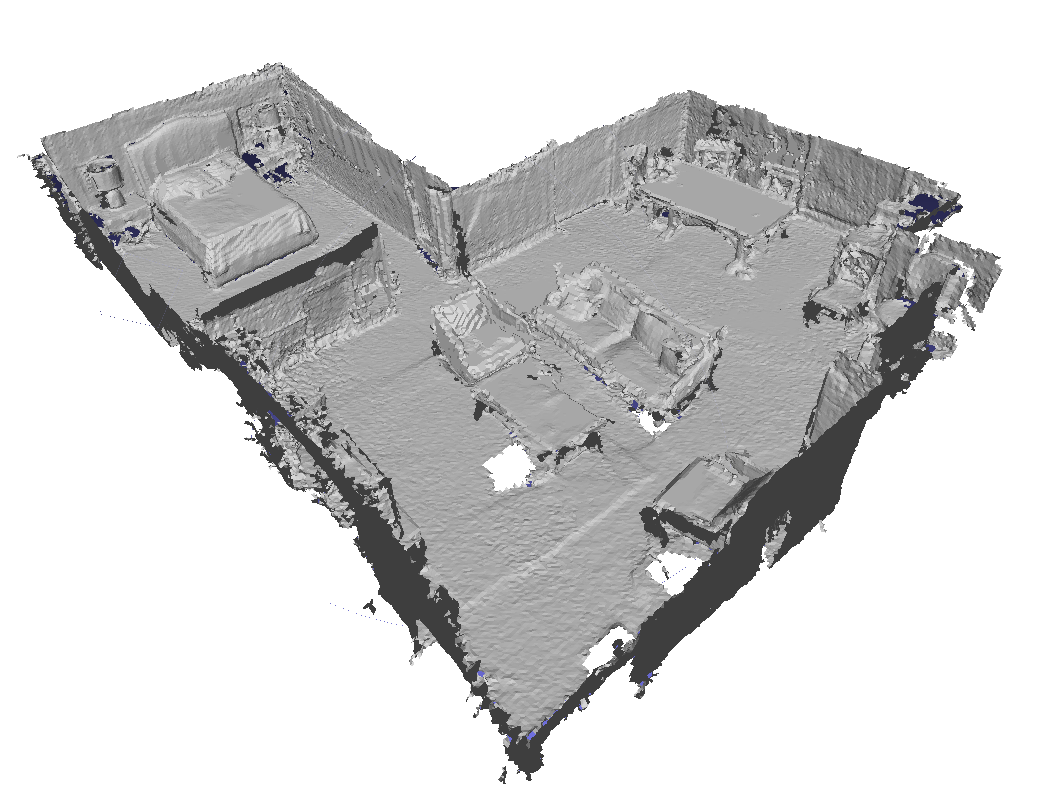
\includegraphics[width=1\textwidth]{img/apartment_scene_nocolor.png}  
% 		 \caption{}
% 		 \label{fig:aparment_nocolor}
% 	 \end{subfigure}
% 	 \begin{subfigure}{0.49\columnwidth} \centering
% 		 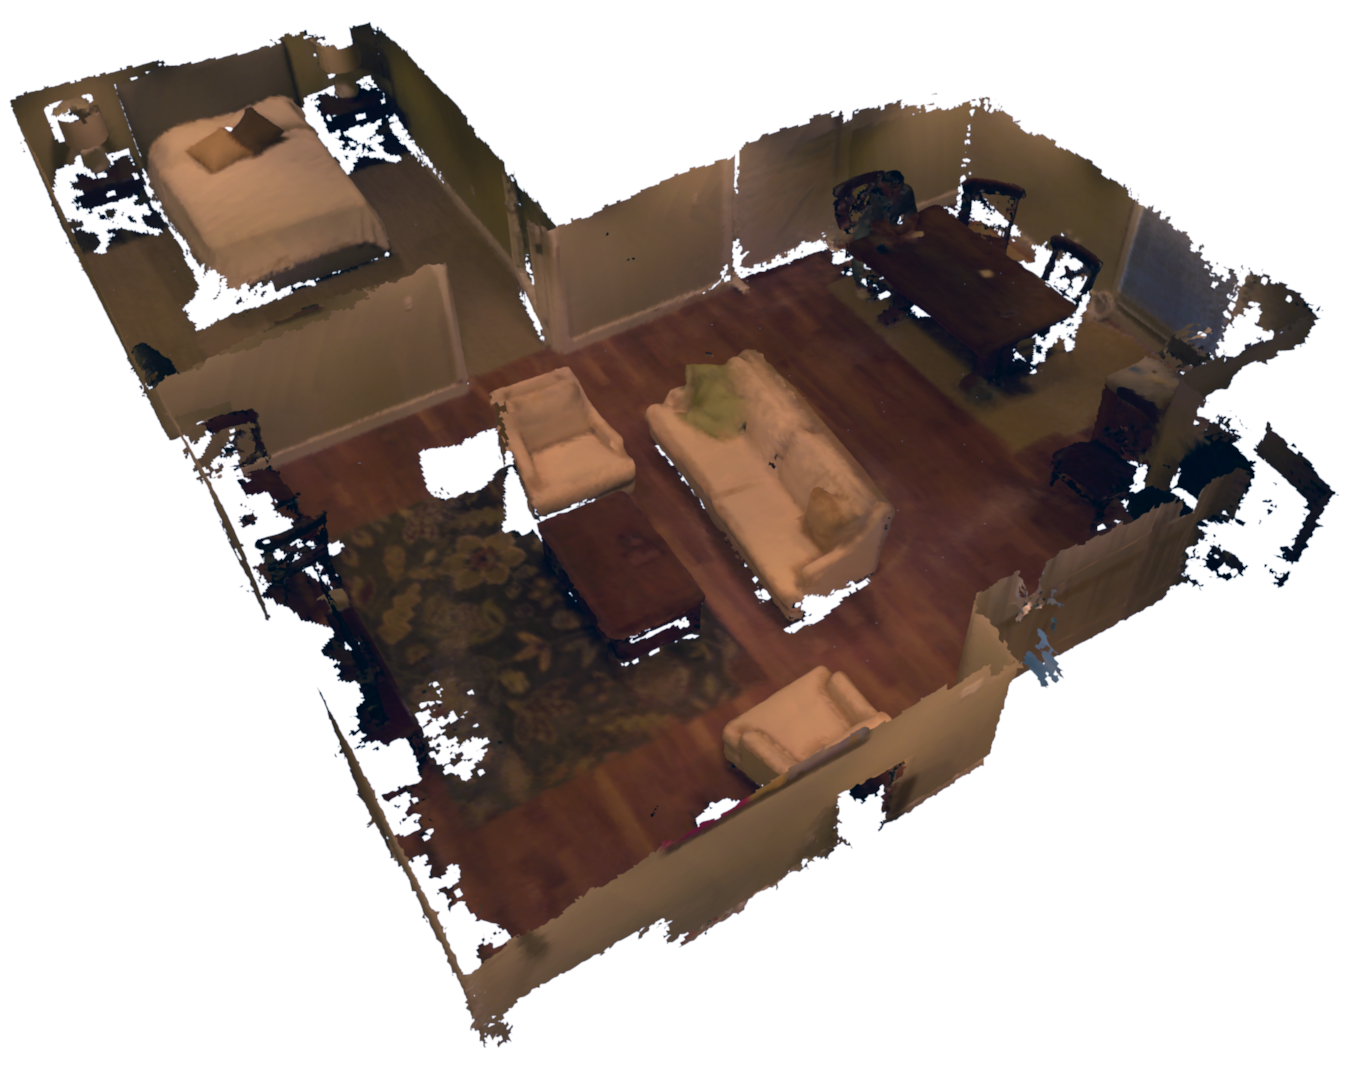
\includegraphics[width=1\textwidth]{img/apartment_scene_color.png}
% 		 \caption{}
% 		 \label{fig:apartment_color}
% 	 \end{subfigure}
% 	 \begin{subfigure} {0.49\columnwidth} \centering
% 		 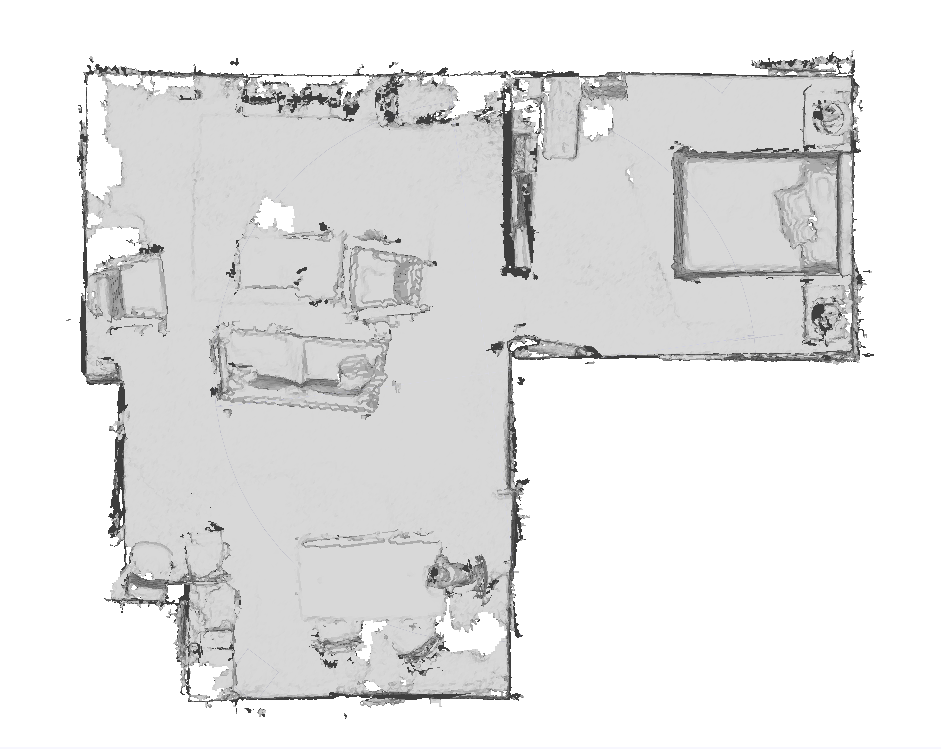
\includegraphics[width=1\textwidth]{img/apartment_scene_topdown_nocolor.png}
% 		 \caption{}
% 		 \label{apartment_scene_topdown_nocolor}
% 	 \end{subfigure}
% 	 \begin{subfigure}{0.49\columnwidth} \centering
% 		 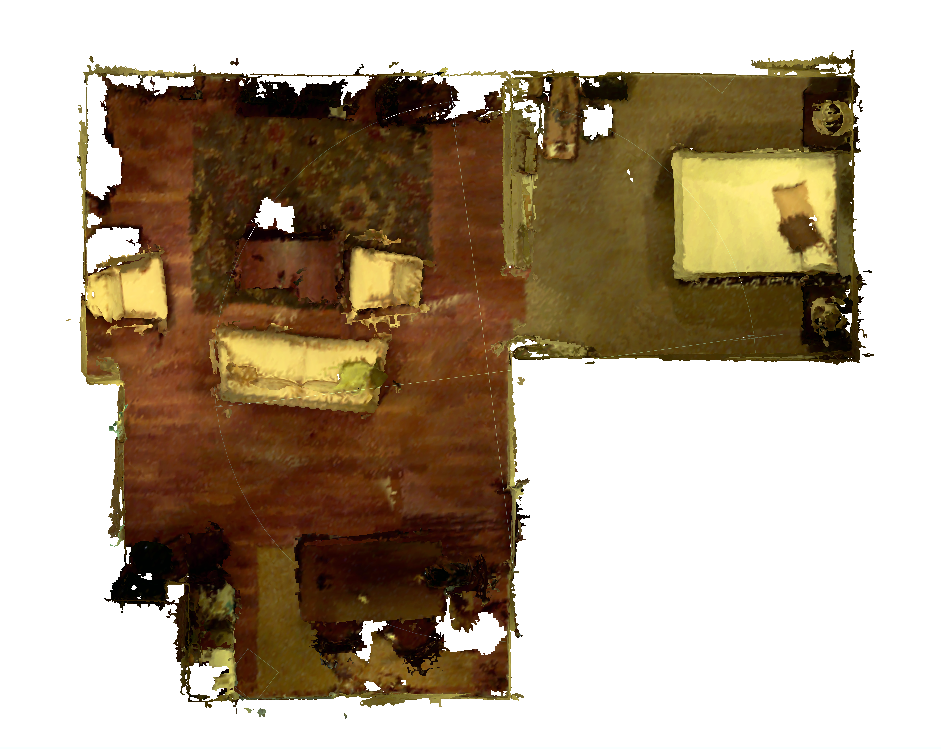
\includegraphics[width=1\textwidth]{img/apartment_scene_topdown_color.png}
% 		 \caption{}
% 		 \label{fig:apartment_scene_topdown_color}
% 	 \end{subfigure}
% % 	 \begin{subfigure} {0.49\columnwidth} \centering
% % 		 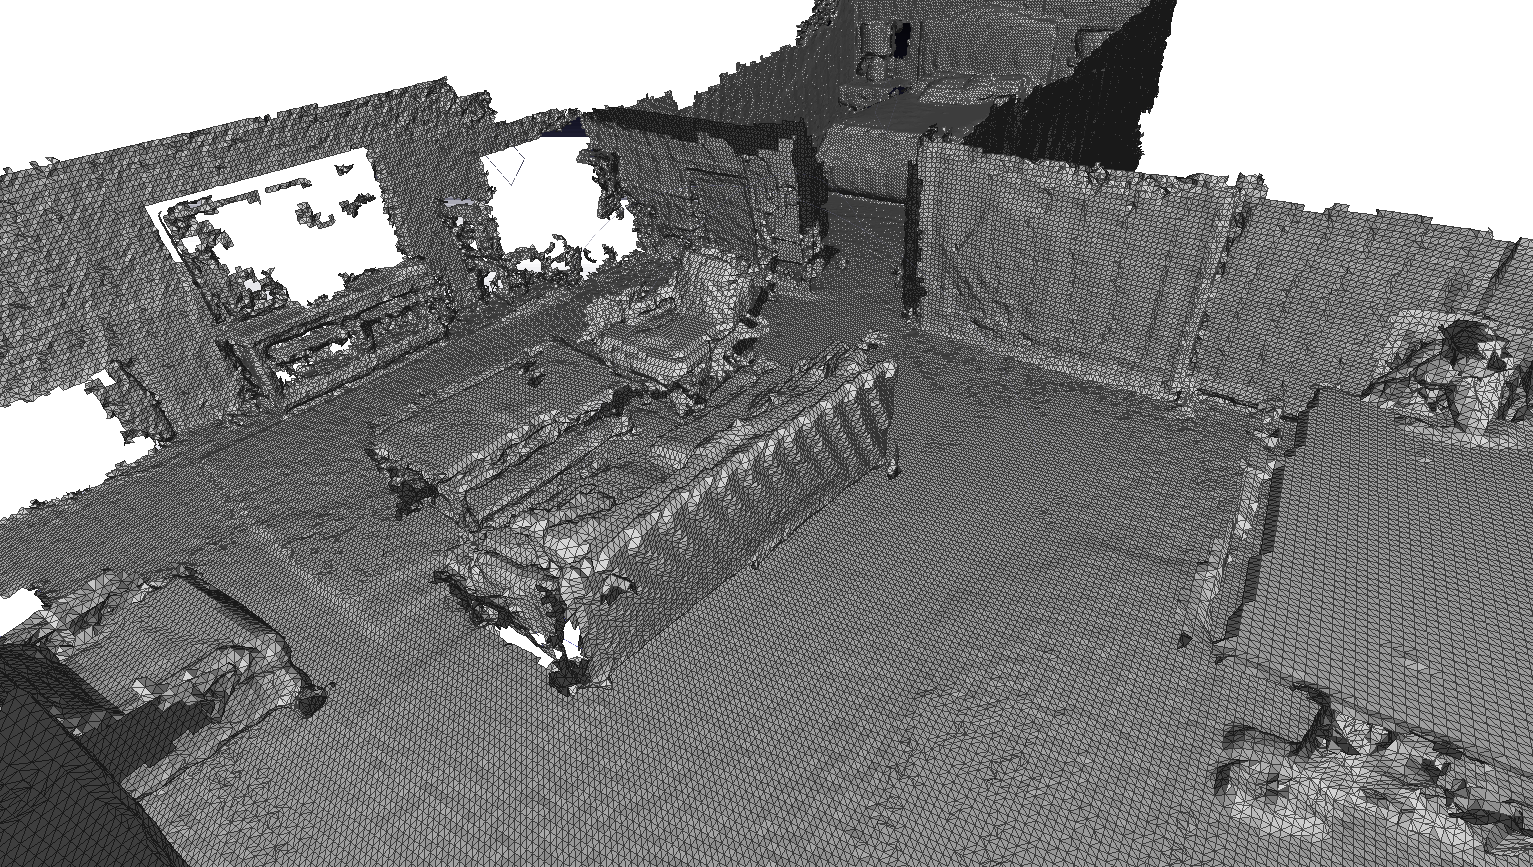
\includegraphics[width=1\textwidth]{img/apartment_scene_closeup_nocolor.png}  
% % 		 \caption{}
% % 		 \label{apartment_scene_closeup_nocolor}
% % 	 \end{subfigure}
% % 	 \begin{subfigure}{0.49\columnwidth} \centering
% % 		 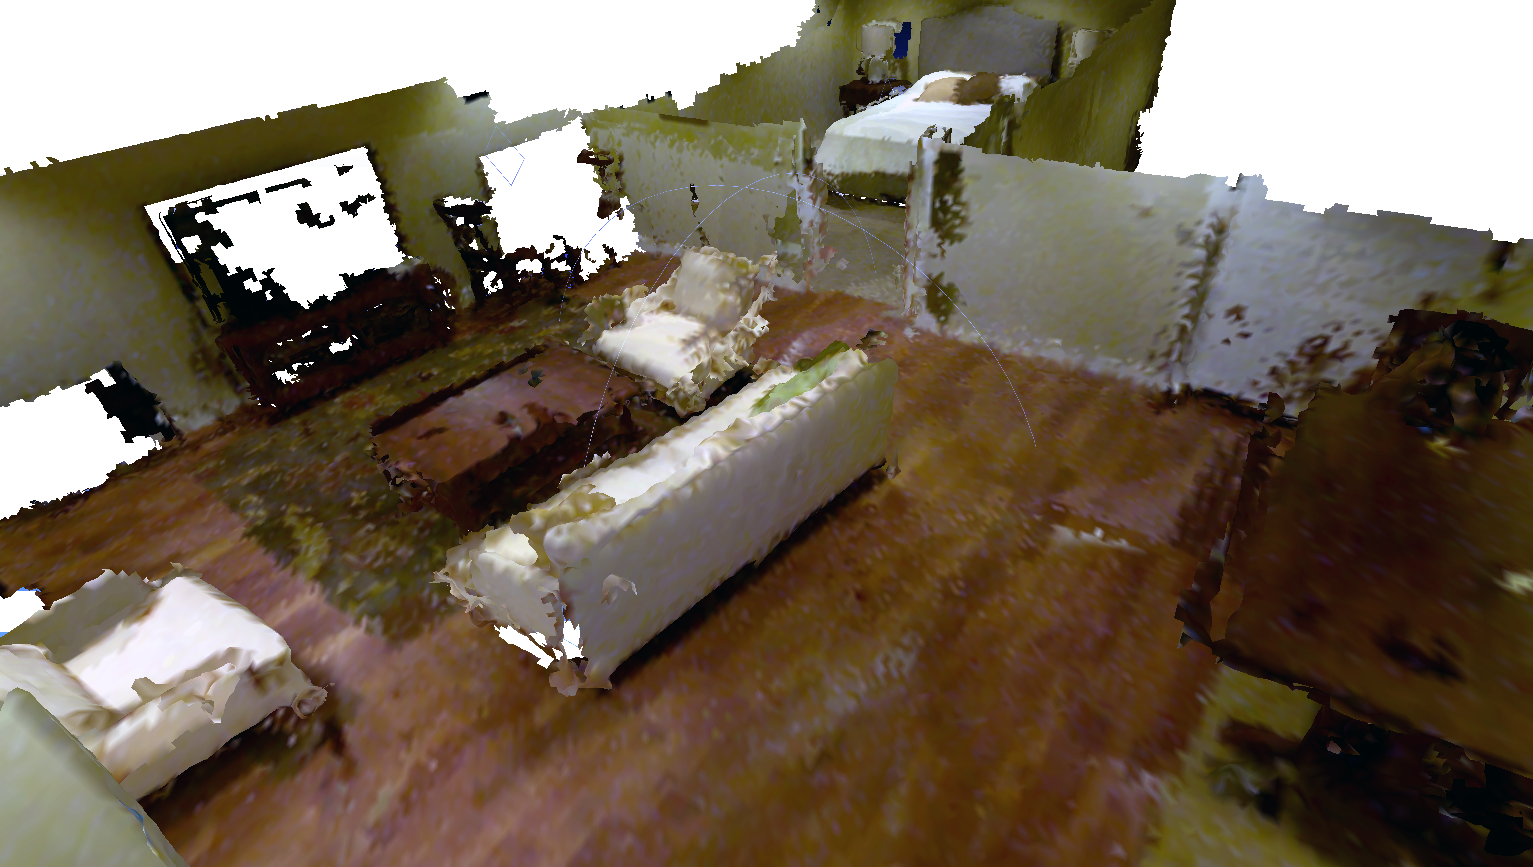
\includegraphics[width=1\textwidth]{img/apartment_scene_closeup_color.png}
% % 		 \caption{}
% % 		 \label{fig:apartment_scene_closeup_color}
% % 	 \end{subfigure}
% 	 \caption{Several views of an apartment scene are shown without and with
% 	 color. These meshes were produced using the tablet device using space
% 	 carving, raycasting, and an offline bundle adjustment procedure to correct
% 	 for pose drift.}
% 	 \label{fig:apartment}
%  \end{figure*}  

%\begin{itemize}
%    \item If we're keeping around the volumetric information, what does that
    % buy us? Can it help us with loop closure?
%    \item These techniques can be used outside of the mobile context to speed
%    things up.
%    \item We gain a lot by using decoupled pose, but there needs to be a way to
 %   incorporate the VIO pose with dense alignment (like they do in Kintinuous).
%\end{itemize}
 
\section{Discussion and Future Work}
Our approach is able to create and render large-scale 3D reconstructions of
scenes in real-time using only the limited computational resources of a
\textit{Tango} device. We accomplish this without any GPU computing, and use
only the fixed function pipeline to render the scene. We do this out of
necessity to meet the computing requirements of a mobile device.

However, the optimizations we have made are equally applicable to other
settings beyond mobile devices. By using a dynamic spatial hash map to store
TSDF data instead of a monolithic array, much larger areas can be
reconstructed. Unlike other approaches which attempt to create large TSDF
reconstructions \cite{Whelan2013}, our approach keeps \textit{all} of the
volumetric information intact. This allows the user to re-visit locations and
improve the reconstruction.

Admittedly, our reconstructions are much lower resolution than state of the art
mapping techniques, which typically push for sub-centimeter resolution. We have
yet to see whether our approach can be combined with GPU solutions to deliver
large-scale, very high resolution reconstructions.One of the biggest
bottlenecks in volumetric integration algorithms is the overhead associated
with transferring data to the GPU. Because of this, all other TSDF-based
approaches (\cite{Newcombe, Whelan2013, Bylow2013, Nguyen2012}) keep only a
fixed amount of memory for the TSDF allocated on the GPU. A fruitful avenue of
future research would be in implementing the dynamic spatial hash map on the GPU
in an efficient way. 

Another area of potential research is in loop closure and pose estimation. Our
approach is purely \textit{open-loop}, taking in pose estimates from visual
odometry as \textit{a prioi} ground truth. Reconstruction can probably be
improved if dense 3D data is used to inform the pose estimator. More
importantly, a means of dealing with global pose estimation using the dense
reconstruction is neeeded. Whelan \etal\cite{WhelanLoopClose} introduced a
means of warping the mesh output by \textit{Kintinuous} consistently with global
pose updates involving loop closures. Can a similar method be used to
\textit{directly} warp the TSDF chunk data to take loop closures into account?

Finally, there is the question of applications. What can be done with a
real-time dense 3D reconstruction on a mobile device? Applications ranging from
robot localization and planning to house-scale modelling and augmented reality
gaming are all possible.

\ifcvprfinal
\section*{Acknowledgements}
This work was done as part of Google's Advanced Technologies and Projects
division (ATAP) for \emph{Project Tango}. Thanks to Johnny Lee, Joel Hesch, Esha
Nerurkar, and Simon Lynen and other ATAP members for their close collaboration
and support on this project. Thanks to Ryan Hickman for collecting outdoor data.
\fi

\bibliographystyle{plain}
% argument is your BibTeX string definitions and bibliography database(s)
\bibliography{densemapping, ./densemapping} 
\end{document}
